%%%%%%%%%%%%%%%%%%%%%%%%%%%%%%%%%%%%%%%%%
% Masters/Doctoral Thesis 
% LaTeX Template
% Version 2.4 (22/11/16)
%
% This template has been downloaded from:
% http://www.LaTeXTemplates.com
%
% Version 2.x major modifications by:
% Vel (vel@latextemplates.com)
%
% This template is based on a template by:
% Steve Gunn (http://users.ecs.soton.ac.uk/srg/softwaretools/document/templates/)
% Sunil Patel (http://www.sunilpatel.co.uk/thesis-template/)
%
% Template license:
% CC BY-NC-SA 3.0 (http://creativecommons.org/licenses/by-nc-sa/3.0/)
%
%%%%%%%%%%%%%%%%%%%%%%%%%%%%%%%%%%%%%%%%%

%----------------------------------------------------------------------------------------
%	PACKAGES AND OTHER DOCUMENT CONFIGURATIONS
%----------------------------------------------------------------------------------------
\documentclass[
11pt, % The default document font size, options: 10pt, 11pt, 12pt
%oneside, % Two side (alternating margins) for binding by default, uncomment to switch to one side
catalan, % ngerman for German
singlespacing, % Single line spacing, alternatives: onehalfspacing or doublespacing
%draft, % Uncomment to enable draft mode (no pictures, no links, overfull hboxes indicated)
%nolistspacing, % If the document is onehalfspacing or doublespacing, uncomment this to set spacing in lists to single
%liststotoc, % Uncomment to add the list of figures/tables/etc to the table of contents
%toctotoc, % Uncomment to add the main table of contents to the table of contents
%parskip, % Uncomment to add space between paragraphs
%nohyperref, % Uncomment to not load the hyperref package
headsepline, % Uncomment to get a line under the header
%chapterinoneline, % Uncomment to place the chapter title next to the number on one line
%consistentlayout, % Uncomment to change the layout of the declaration, abstract and acknowledgements pages to match the default layout
table
]{MastersDoctoralThesis} % The class file specifying the document structure

\usepackage[utf8]{inputenc} % Required for inputting international characters
\usepackage[T1]{fontenc} % Output font encoding for international characters

\usepackage{palatino} % Use the Palatino font by default

\usepackage[backend=bibtex,style=authoryear,natbib=true]{biblatex} % Use the bibtex backend with the authoryear citation style (which resembles APA)
\usepackage{eurosym}


\addbibresource{example.bib} % The filename of the bibliography

\usepackage[autostyle=true]{csquotes} % Required to generate language-dependent quotes in the bibliography

%----------------------------------------------------------------------------------------
%	MARGIN SETTINGS
%----------------------------------------------------------------------------------------

\geometry{
	paper=a4paper, % Change to letterpaper for US letter
	inner=2.5cm, % Inner margin
	outer=3.8cm, % Outer margin
	bindingoffset=.5cm, % Binding offset
	top=1.5cm, % Top margin
	bottom=1.5cm, % Bottom margin
	%showframe, % Uncomment to show how the type block is set on the page
}

%----------------------------------------------------------------------------------------
%	THESIS INFORMATION
%----------------------------------------------------------------------------------------

\thesistitle{Sistema de monitoratge autoadaptable heterogeni i distribuït} % Your thesis title, this is used in the title and abstract, print it elsewhere with \ttitle
\supervisor{Xavier \textsc{Franch Gutierrez}} % Your supervisor's name, this is used in the title page, print it elsewhere with \supname
\examiner{Marc \textsc{Oriol Hilari}} % Your examiner's name, this is not currently used anywhere in the template, print it elsewhere with \examname
\degree{Grau d'Enginyeria Informàtica} % Your degree name, this is used in the title page and abstract, print it elsewhere with \degreename
\author{Joaquim \textsc{Motger de la Encarnación}} % Your name, this is used in the title page and abstract, print it elsewhere with \authorname
\addresses{} % Your address, this is not currently used anywhere in the template, print it elsewhere with \addressname

\subject{} % Your subject area, this is not currently used anywhere in the template, print it elsewhere with \subjectname
\keywords{} % Keywords for your thesis, this is not currently used anywhere in the template, print it elsewhere with \keywordnames
\university{{Universitat Politècnica de Catalunya}} % Your university's name and URL, this is used in the title page and abstract, print it elsewhere with \univname
\department{{Enginyeria de Serveis i Sistemes de la Informació}} % Your department's name and URL, this is used in the title page and abstract, print it elsewhere with \deptname
\group{{Enginyeria del Software}} % Your research group's name and URL, this is used in the title page, print it elsewhere with \groupname
\faculty{{Facultat d'Informàtica de Barcelona}} % Your faculty's name and URL, this is used in the title page and abstract, print it elsewhere with \facname

\AtBeginDocument{
\hypersetup{pdftitle=\ttitle} % Set the PDF's title to your title
\hypersetup{pdfauthor=\authorname} % Set the PDF's author to your name
\hypersetup{pdfkeywords=\keywordnames} % Set the PDF's keywords to your keywords
}

\begin{document}

\frontmatter % Use roman page numbering style (i, ii, iii, iv...) for the pre-content pages

\pagestyle{plain} % Default to the plain heading style until the thesis style is called for the body content

%----------------------------------------------------------------------------------------
%	TITLE PAGE
%----------------------------------------------------------------------------------------

\begin{titlepage}
\begin{center}

%\vspace*{.06\textheight}

\includegraphics[width=\textwidth]{fib.png}\vspace{4.0cm} % University/department logo - uncomment to place it
%{\scshape\LARGE \univname\par}\vspace{1.5cm} % University name
%\textsc{\Large Treball de Final de Grau}\\[1.5cm] % Thesis type

\HRule \\[0.4cm] % Horizontal line
{\huge \bfseries \ttitle\par}\vspace{0.4cm} % Thesis title
\HRule \\[1.5cm] % Horizontal line
 
\begin{minipage}[t]{0.4\textwidth}
\begin{flushleft} \large
\emph{Autor:}\\
\href{}{\authorname} % Author name - remove the \href bracket to remove the link
\end{flushleft}
\end{minipage}
\begin{minipage}[t]{0.4\textwidth}
\begin{flushright} \large
\emph{Director:} \\
\href{}{\supname} % Supervisor name - remove the \href bracket to remove the link  
\end{flushright}
\begin{flushright} \large
\emph{Codirector:} \\
\href{}{\examname} % Supervisor name - remove the \href bracket to remove the link  
\end{flushright}
\end{minipage}\\[6cm]
 
%\vfill

\large \textit{Treball de final de grau presentat sota el marc del}\\[0.3cm] % University requirement text
\degreename\\[0.5cm]
\textit{en l'especialitat de}\\[0.3cm]
\groupname\\[2cm] % Research group name and department name
 
%\vfill
 
\vfill
\end{center}
\end{titlepage}

%----------------------------------------------------------------------------------------
%	DECLARATION PAGE
%----------------------------------------------------------------------------------------
%
%\begin{declaration}
%\addchaptertocentry{\authorshipname} % Add the declaration to the table of contents
%\noindent Jo, \authorname, declaro que aquest Treball de Final de Grau titulat \textit{\ttitle}
%i el treball presentats en el mateix són propis. Declaro que:

%\begin{itemize} 
%\item La feina aquí presentada ha estat desenvolupada durant el curs del Grau en Enginyeria Informàtica
%\item S'ha indicat degudament l'ús de publicacions o components d'autoria externa, utilitzats com a suport pel desenvolupament del projecte, reconeixent l'autoria original dels mateixos
%\item S'ha indicat degudament tota la feina desenvolupada per autoria pròpia
%\item Totes les publicacions terceres consultades pel desenvolupament del treball estan degudament citades
%\item \\
%\end{itemize}
%\noindent I per deixar constància d'aquesta declaració, signo el present document\\[2cm]
 
%\noindent Signatura:\\
%\rule[2cm]{25em}{0.5pt} % This prints a line for the signature
% 
%\noindent Date:\\
%\rule[0.5em]{25em}{0.5pt} % This prints a line to write the date
%\end{declaration}

%----------------------------------------------------------------------------------------
%	QUOTATION PAGE
%----------------------------------------------------------------------------------------

%\vspace*{0.2\textheight}

%\noindent{\itshape A mi madre, quien me dio las herramientas para ser capaz de hacer camino al andar.}\bigbreak

%----------------------------------------------------------------------------------------
%	ABSTRACT PAGE
%----------------------------------------------------------------------------------------

\begin{Abstracte}
\addchaptertocentry{Abstracte} % Add the abstract to the table of contents
El monitoratge consisteix en la tècnica d'observació i control dels sistemes software amb l'objectiu de garantir la seva fiabilitat, la qualitat del servei (Quality of Service, QoS), la seguretat i altres característiques dels sistemes software pròpies de la seva execució en temps real. El monitoratge proporciona la informació que permet a un sistema software autoadaptable modificar la seva execució davant la violació d'uns certs valors sobre aquestes característiques. De la mateixa manera, els sistemes de monitoratge requereixen també poder adaptar la seva execució per satisfer la seva fiabilitat. En aquest context, com podem dotar a un sistema de monitoratge de capacitats autoadaptables?\\

En base a aquesta premisa, aquest Treball de Final de Grau consisteix en el disseny i implementació d'un sistema de monitoratge autoadaptable, heterogeni i distribuït que integra un conjunt de monitors de naturalesa diversa i permet, mitjançant la gestió i adaptació de diagrames UML, la seva reconfiguració de forma automàtica. La proposta i el desenvolupament plantejats en aquest projecte es validen mitjançant casos d'ús reals i, en especial èmfasi, amb la seva integració dins el marc de SUPERSEDE, un projecte del programa Horizon 2020 enfocat a la gestió del cicle de vida dels serveis software i les aplicacions, amb l'objectiu de millorar l'experiència final de l'usuari en l'ús d'aquests sistemes. 
\end{Abstracte}

%----------------------------------------------------------------------------------------
%	ACKNOWLEDGEMENTS
%----------------------------------------------------------------------------------------

%\begin{acknowledgements}
%\addchaptertocentry{\acknowledgementname} % Add the acknowledgements to the table of contents
%The acknowledgments and the people to thank go here, don't forget to include your project advisor\ldots
%\end{acknowledgements}

%----------------------------------------------------------------------------------------
%	LIST OF CONTENTS/FIGURES/TABLES PAGES
%----------------------------------------------------------------------------------------

\tableofcontents % Prints the main table of contents

\listoffigures % Prints the list of figures

\listoftables % Prints the list of tables

%----------------------------------------------------------------------------------------
%	ABBREVIATIONS
%----------------------------------------------------------------------------------------

%\begin{abbreviations}{ll} % Include a list of abbreviations (a table of two columns)

%\textbf{LAH} & \textbf{L}ist \textbf{A}bbreviations \textbf{H}ere\\
%\textbf{WSF} & \textbf{W}hat (it) \textbf{S}tands \textbf{F}or\\

%\end{abbreviations}

%----------------------------------------------------------------------------------------
%	PHYSICAL CONSTANTS/OTHER DEFINITIONS
%----------------------------------------------------------------------------------------

%\begin{constants}{lr@{${}={}$}l} % The list of physical constants is a three column table

% The \SI{}{} command is provided by the siunitx package, see its documentation for instructions on how to use it

%Speed of Light & $c_{0}$ & \SI{2.99792458e8}{\meter\per\second} (exact)\\
%Constant Name & $Symbol$ & $Constant Value$ with units\\

%\end{constants}

%----------------------------------------------------------------------------------------
%	SYMBOLS
%----------------------------------------------------------------------------------------

%\begin{symbols}{lll} % Include a list of Symbols (a three column table)

%$a$ & distance & \si{\meter} \\
%$P$ & power & \si{\watt} (\si{\joule\per\second}) \\
%Symbol & Name & Unit \\

%\addlinespace % Gap to separate the Roman symbols from the Greek

%$\omega$ & angular frequency & \si{\radian} \\

%\end{symbols}

%----------------------------------------------------------------------------------------
%	DEDICATION
%----------------------------------------------------------------------------------------

%\dedicatory{For/Dedicated to/To my\ldots} 

%----------------------------------------------------------------------------------------
%	THESIS CONTENT - CHAPTERS
%----------------------------------------------------------------------------------------

\mainmatter % Begin numeric (1,2,3...) page numbering

\pagestyle{thesis} % Return the page headers back to the "thesis" style

% Include the chapters of the thesis as separate files from the Chapters folder
% Uncomment the lines as you write the chapters

% Chapter Template

\chapter{Introducció} % Main chapter title

\label{Introduccio} % Change X to a consecutive number; for referencing this chapter elsewhere, use \ref{ChapterX}

El present document consisteix en la memòria del Treball de Final de Grau (TFG) del Grau en Enginyeria Informàtica titulat \textit{Sistema de monitoratge autoadaptable, heterogeni i distribuït}. Aquest TFG s'ha realitzat com a part dels estudis en l'especialitat d'Enginyeria del Software, i per tant els coneixements i les tasques aquí resumits s'emmarquen en els conceptes d'aquesta àrea.

\section{Motivació del projecte}

Com a projecte realitzat a la cloenda dels estudis de grau, el desenvolupament i presentació d'aquest projecte tenen dos objectius principals.\\

En primer lloc, la consolidació dels coneixements adquirits durant el transcurs del grau. Aquests coneixements engloben des de la qüestió tècnica i específica de la matèria, amb especial èmfasi en els conceptes i aprenentatges relacionats amb l'especialitat d'Enginyeria del Software (tals com el disseny de components software), fins a aspectes relacionats amb la gestió, realització i documentació de projectes complets, pràctics i funcionals, dels quals aquest TFG n'és un exemple. Al llarg dels capítols que componen aquesta memòria, la justificació, explicació i demostració de les tasques realitzades i els conceptes tractats s'exposen amb la rigorositat adequada a un document acadèmic d'aquesta categoria, demostrant l'assoliment d'aquests coneixements amb la major claredat possible.\\

Per altra banda, aquest projecte pretén presentar-se com un treball d'investigació, recerca i desenvolupament amb valor propi, dins d'un àmbit i context determinats, amb un objectiu pràctic i aplicable. Més enllà del caire acadèmic, els productes i resultats generats com a conseqüència de la realització d'aquest projecte (components software, disseny i implementació de sistemes, documentació, etc.) esdevenen elements amb valor propi, amb expectatives d'ús  i possibilitats d'expansió dins del seu propi context.\\

Per tal de satisfer aquests dos objectius, aquest projecte presenta el següent propòsit: dissenyar, implementar, gestionar, testejar, validar i mantenir un sistema de monitoratge que satisfaci els criteris d'autoadaptabilitat, heterogeneïtat i distribució (conceptes que s'aprofundiran més endavant). Sota aquesta temàtica, i amb les consideracions prèviament establertes, s'assoliran tant l'objectiu de consolidació de coneixements com la generació d'uns resultats que puguin ser presentats pel seu valor propi i independent.\\

Per tal d'entendre bé aquest plantejament de propòsit general del projecte, a continuació detallarem una breu definició de les bases de l'àrea de treball sobre la qual aquest projecte n'és un desenvolupament.

\section{Àrea d'estudi i justificació de la temàtica}

En les darreres dècades els sistemes software han evolucionat fins al punt d'esdevenir elements clau i imprescindibles de les activitats primàries de qualsevol empresa, organització o institució. La gestió de la informació, els protocols i controls de seguretat, els processos de negoci, etc., són els reptes als quals els \textit{Chief Information Officers} (CIO) de moltes empreses s'han d'enfrontar. Aquests reptes i els seus resultats depenen, en gran mesura, del comportament dels sistemes software que entren en joc dins aquestes activitats. Addicionalment, la quantitat de productes software exposats com a serveis o aplicacions mòbils ha incrementat dràsticament. Fet que deriva en el sorgiment d'una gran varietat de contexts i entorns d'execució entre els grans volums d'usuaris que aquests sistemes poden tenir. \\

És per aquest motiu que eventualment ha anat prenent força un concepte basat en l'estudi i control de qualitat dels sistemes software: el monitoratge. Com a part de la vida professional d'un enginyer de software, la supervisió i control dels components i sistemes amb els què treballa és un concepte clau amb el qual, d'una forma o altra, ha d'estar familiaritzat. Però el problema que plantegem aquí va més enllà: després del repte de monitorar els sistemes, ens hem de plantejar com dissenyar, gestionar i adaptar aquest monitoratge.\\

Els reptes que aquestes tasques plantegen i que aquest projecte treballa són diversos. Entre d'altres, cal valorar el disseny i les característiques tècniques dels monitors, la seva configuració i la capacitat d'adaptabilitat. En relació amb aquest últim aspecte, també cal valorar com s'emmagatzemen i es gestionen els detalls relacionats amb la configuració dels monitors, i establir interaccions de la manera més genèrica possible per facilitar l'extensibilitat.\\

Existeix una àmplia recerca que actualment treballa i desenvolupa projectes en relació a aquest àmbit. El potencial d'estudi que ofereix resulta d'un alt interès a causa de la possibilitat de recerca i síntesi i als diferents aspectes i criteris sobre els quals es pot treballar.\\

Així, tant com estudiant com a futur professional del sector de l'enginyeria del software, es poden contemplar diversos criteris per treballar en aquesta temàtica:
\begin{itemize}
\item Un aprofundiment en els coneixements de l'enginyeria i els sistemes software
\item Treball i recerca en conceptes de control de qualitat, fiabilitat i millora de l'experiència de l'usuari
\item Possibilitat de col·laborar i aprofundir en un tema de recerca d'actualitat dins l'enginyeria de serveis i els sistemes d'informació
\item Plantejament d'un projecte complet que pugui servir a tercers interessats en l'estudi de sistemes de monitoratge autoadaptatius
\end{itemize}  

\section{Identificació de potencials stakeholders}

Les diferents fases que engloben aquest projecte deriven en l'obtenció d'un producte final, orientat a la seva aplicació pràctica. Com a tal, els documents generats i els components dissenyats i implementats esdevenen productes propis dins el context del monitoratge de sistemes software. Com a tals, aspectes que s'exposaran al llarg d'aquest document (el disseny i implementació d'una arquitectura genèrica pels monitors, la gestió de les configuracions, etc.) poden resultar d'utilitat per a agents externs a la pròpia autoria del projecte.\\

Podem considerar, per tant, que podrà ser una eina d’interès pels principals stakeholders, que vindrien a ser:
\begin{itemize}
\item \textbf{Desenvolupadors i enginyers software}. Aquells agents al càrrec del control de qualitat de sistemes softwares de diverses naturaleses. Els conceptes treballats, el plantejament de problemàtiques, i el producte generat, poden aportar valor de qualitat al sector treballant, per una banda, en la síntesi i recopilació de la informació actual, i per altra banda, aportant propostes i solucions pròpies basades en l’experiència del desenvolupament del projecte.
\item \textbf{Gestors de projecte i experts en Sistemes d'Informació}. La gestió de la informació, el tractament i el seu potencial poden resultar afectats gràcies a la capacitat de recol·lecció de dades del sistema de monitoratge, així com els criteris de revisió i control de qualitat, que permeten analitzar i obtenir informació fiable.
\item \textbf{Usuaris finals dels sistemes monitorats}. De forma indirecta, es veuran afectats degut a les conseqüències del monitoratge dut a terme per aquest sistema de monitoratge o d’altres derivats dels conceptes treballats al llarg d’aquest projecte.
\end{itemize}

En definitiva, podem concloure que l'àrea de treball del projecte té potencial per ser d'interès i tenir una reaprofitabilitat, factor clau que explotarem al llarg del disseny i desenvolupament d'aquest projecte. 
% Chapter Template

\chapter{Contextualització} % Main chapter title

\label{Contextualitzacio} % Change X to a consecutive number; for referencing this chapter elsewhere, use \ref{ChapterX}

%----------------------------------------------------------------------------------------
%	SECTION 1
%----------------------------------------------------------------------------------------

\section{Justificació de la temàtica}

Lorem ipsum dolor sit amet, consectetur adipiscing elit. Aliquam ultricies lacinia euismod. Nam tempus risus in dolor rhoncus in interdum enim tincidunt. Donec vel nunc neque. In condimentum ullamcorper quam non consequat. Fusce sagittis tempor feugiat. Fusce magna erat, molestie eu convallis ut, tempus sed arcu. Quisque molestie, ante a tincidunt ullamcorper, sapien enim dignissim lacus, in semper nibh erat lobortis purus. Integer dapibus ligula ac risus convallis pellentesque.

%-----------------------------------
%	SUBSECTION 1
%-----------------------------------
\section{Definició de l'àrea d'estudi}

Nunc posuere quam at lectus tristique eu ultrices augue venenatis. Vestibulum ante ipsum primis in faucibus orci luctus et ultrices posuere cubilia Curae; Aliquam erat volutpat. Vivamus sodales tortor eget quam adipiscing in vulputate ante ullamcorper. Sed eros ante, lacinia et sollicitudin et, aliquam sit amet augue. In hac habitasse platea dictumst.

%-----------------------------------
%	SUBSECTION 2
%-----------------------------------

\subsection{Identificació dels stakeholders}
Morbi rutrum odio eget arcu adipiscing sodales. Aenean et purus a est pulvinar pellentesque. Cras in elit neque, quis varius elit. Phasellus fringilla, nibh eu tempus venenatis, dolor elit posuere quam, quis adipiscing urna leo nec orci. Sed nec nulla auctor odio aliquet consequat. Ut nec nulla in ante ullamcorper aliquam at sed dolor. Phasellus fermentum magna in augue gravida cursus. Cras sed pretium lorem. Pellentesque eget ornare odio. Proin accumsan, massa viverra cursus pharetra, ipsum nisi lobortis velit, a malesuada dolor lorem eu neque.

%----------------------------------------------------------------------------------------
%	SECTION 2
%----------------------------------------------------------------------------------------

\section{Estat de l'art}

Sed ullamcorper quam eu nisl interdum at interdum enim egestas. Aliquam placerat justo sed lectus lobortis ut porta nisl porttitor. Vestibulum mi dolor, lacinia molestie gravida at, tempus vitae ligula. Donec eget quam sapien, in viverra eros. Donec pellentesque justo a massa fringilla non vestibulum metus vestibulum. Vestibulum in orci quis felis tempor lacinia. Vivamus ornare ultrices facilisis. Ut hendrerit volutpat vulputate. Morbi condimentum venenatis augue, id porta ipsum vulputate in. Curabitur luctus tempus justo. Vestibulum risus lectus, adipiscing nec condimentum quis, condimentum nec nisl. Aliquam dictum sagittis velit sed iaculis. Morbi tristique augue sit amet nulla pulvinar id facilisis ligula mollis. Nam elit libero, tincidunt ut aliquam at, molestie in quam. Aenean rhoncus vehicula hendrerit.

%-----------------------------------
%	SUBSECTION 2
%-----------------------------------

\subsection{Projecte SUPERSEDE}
Morbi rutrum odio eget arcu adipiscing sodales. Aenean et purus a est pulvinar pellentesque. Cras in elit neque, quis varius elit. Phasellus fringilla, nibh eu tempus venenatis, dolor elit posuere quam, quis adipiscing urna leo nec orci. Sed nec nulla auctor odio aliquet consequat. Ut nec nulla in ante ullamcorper aliquam at sed dolor. Phasellus fermentum magna in augue gravida cursus. Cras sed pretium lorem. Pellentesque eget ornare odio. Proin accumsan, massa viverra cursus pharetra, ipsum nisi lobortis velit, a malesuada dolor lorem eu neque.
% Chapter Template

\chapter{Objectius} % Main chapter title

\label{Objectius} % Change X to a consecutive number; for referencing this chapter elsewhere, use \ref{ChapterX}

%----------------------------------------------------------------------------------------
%	SECTION 1
%----------------------------------------------------------------------------------------

Definit el context, l'àrea d'estudi i una aproximació a l'estat de l'art actual d'aquest projecte, cal definir amb el màxim nivell de detall quins seran els objectius principals, així com els objectius específics i l'abast, per tal d'introduïr els conceptes treballats durant el desenvolupament del mateix.

\section{Objectiu general}

L’objectiu principal d’aquest projecte consisteix en la implementació d’un sistema software orientat al monitoratge d’altres sistemes softwares. Aquest sistema haurà de complir 3 característiques principals: ser autoadaptable, heterogeni i distribuït. A continuació procedim a explicar en detall què entendrem per aquestes característiques dins el context d’aquest projecte, en base a la contextualització i els conceptes explicats anteriorment:

\begin{enumerate}
\item \textbf{Autoadaptable}. El sistema de monitoratge generat ha d'estar dotat de capacitats d'adaptabilitat de la seva execució en temps real. Mitjançant la gestió i control de la seva activitat, els diferents monitors han d'oferir eines d'adaptació orientades al control de qualitat del propi sistema. Per fer-ho, caldrà tenir en compte dos punts que es desenvoluparan més endavant: en primer lloc, la dotació dels monitors d'aquestes eines d'adaptació; en segon lloc, el disseny i implementació dels components necessaris per gestionar les adaptacions.
\item \textbf{Heterogeni}. El sistema constarà d’un conjunt de monitors de naturalesa variada i permetrà, mitjançant un disseny i una arquitectura prou genèrica, la integració de nous monitors de diversa índole. Per tant, el sistema haurà d’estar capacitat per gestionar els diversos tipus de monitors tot i les seves diferències en aspectes com el sistema monitorat, la naturalesa del monitoratge, les necessitats de configuració, etc. L'objectiu d'aquesta característica és que el resultat final sigui el més aprofitable i reusable possible.
\item \textbf{Distribuït}. El sistema haurà de permetre desplegar els diferents monitors i els components d'adaptabilitat de forma distribuïda i, per tant, tenir la capacitat de desplegar els diferents components com a elements independents dins el nostre sistema genèric.
\end{enumerate}

Els detalls tècnics de l'assoliment d'aquests 3 objectius es desenvoluparan al llarg d'aquesta memòria. 

%-----------------------------------
%	SUBSECTION 1
%-----------------------------------
\subsection{Objectius específics}

En base a l’objectiu general prèviament establert, cal definir una sèrie d’objectius específics que ens permetran assolir-lo definint unes vies prou clares com per a facilitar el desenvolupament del projecte. Procedim, doncs, a enumerar aquests objectius:

\begin{itemize}
\item \textbf{OBJ1.} Definir una planificació pel desenvolupament del projecte en funció dels requisits.
\item \textbf{OBJ2.} Dissenyar una arquitectura software adequada a les necessitats.
\item \textbf{OBJ3.} Implementar el sistema de monitoratge.
\item \textbf{OBJ4.} Implementar el sistema d'adaptació dels monitors.
\item \textbf{OBJ5.} Generació d’un producte final usable, que pugui ser desplegable i reproduïble en format demo.
\item \textbf{OBJ6.} Configurar i definir l’entorn de desenvolupament i d’ús del sistema.
\item \textbf{OBJ7.} Assegurar qualitat i fiabilitat mitjançant els criteris definits.
\item \textbf{OBJ8.} Seguir una metodologia de desenvolupament i testing del sistema.
\item \textbf{OBJ9.} Definir una sèrie de casos d’ús per mostrar la usabilitat i comportament real del sistema.
\item \textbf{OBJ10.} Documentar i justificar l’evolució del projecte.
\end{itemize}

Aquests objectius engloben les dues vessants d'aquest projecte, ja especificades anteriorment: la generació i documentació d'un Treball de Final de Grau, i el disseny i la implementació del sistema descrit. En qualsevol cas, aquests objectius específics defineixen les "metes finals" d'aquest projecte. Per garantir-ne i comprendre el desenvolupament fins a assolir-los, cal definir les tasques i, per tant, l'abast específic d'aquest projecte.

%----------------------------------------------------------------------------------------
%	SECTION 2
%----------------------------------------------------------------------------------------

\section{Abast del projecte}

Els objectius específics prèviament identificats ens donen una visió acurada de l’abast del nostre projecte i les tasques a realitzar. Tot i així, és important reflectir de forma explícita l’abast d’aquest projecte, enumerant els requisits (o dit d’una altra manera, les tasques o necessitats a satisfer) i delimitant el nostre projecte. Ens basarem per tant en els següents punts:

\begin{itemize}
\item Realitzar una recerca bibliogràfica (basada en l’estat de l’art) per assentar les bases i el context del desenvolupament del projecte.
\item Dissenyar, implementar i documentar un disseny arquitectònic software que satisfaci l’objectiu general i els tres criteris (autoadaptabilitat, heterogeneïtat i distribució) del nostre sistema de monitoratge.
\item Dissenyar, implementar i documentar el sistema d'adaptabilitat dels monitors i realitzar la integració amb els mateixos.
\item Definir una sèrie de casos d'ús (mínim de 3 escenaris) que ens permetin validar les funcionalitats del sistema amb exemples mitjançant l'execució real.
\item Dissenyar i implementar un dashboard que permeti visualitzar l'activitat del sistema de monitoratge i adaptabilitat.
\end{itemize}

Aquests punts estableixen el mínim del que podríem considerar com a necessari per considerar que s’han assolit els objectius esmentats a l’apartat 3 d’aquest document. Tot i així, podem preveure la possibiltiat de permetre’ns augmentar les perspectives, i gràcies a l’ús d’una metodologia àgil (veure apartat 5.1. Metodologia de treball), augmentar l’abast del projecte, amb aspectes com incrementar el nombre de monitors implementats, o augmentar les funcionalitats del dashboard. En qualsevol cas, aquests aspectes serien un afegit secundari que únicament tindrà sentit contemplar amb el transcurs del projecte. 
% Chapter Template

\chapter{Gestió i desenvolupament} % Main chapter title

\label{GestioIDesenvolupament} % Change X to a consecutive number; for referencing this chapter elsewhere, use \ref{ChapterX}

%----------------------------------------------------------------------------------------
%	SECTION 1
%----------------------------------------------------------------------------------------

\section{Metodologia de desenvolupament}

Lorem ipsum dolor sit amet, consectetur adipiscing elit. Aliquam ultricies lacinia euismod. Nam tempus risus in dolor rhoncus in interdum enim tincidunt. Donec vel nunc neque. In condimentum ullamcorper quam non consequat. Fusce sagittis tempor feugiat. Fusce magna erat, molestie eu convallis ut, tempus sed arcu. Quisque molestie, ante a tincidunt ullamcorper, sapien enim dignissim lacus, in semper nibh erat lobortis purus. Integer dapibus ligula ac risus convallis pellentesque.

%-----------------------------------
%	SUBSECTION 1
%-----------------------------------
\section{Planificació temporal}

Nunc posuere quam at lectus tristique eu ultrices augue venenatis. Vestibulum ante ipsum primis in faucibus orci luctus et ultrices posuere cubilia Curae; Aliquam erat volutpat. Vivamus sodales tortor eget quam adipiscing in vulputate ante ullamcorper. Sed eros ante, lacinia et sollicitudin et, aliquam sit amet augue. In hac habitasse platea dictumst.

%-----------------------------------
%	SUBSECTION 2
%-----------------------------------

\section{Viabilitat}
Morbi rutrum odio eget arcu adipiscing sodales. Aenean et purus a est pulvinar pellentesque. Cras in elit neque, quis varius elit. Phasellus fringilla, nibh eu tempus venenatis, dolor elit posuere quam, quis adipiscing urna leo nec orci. Sed nec nulla auctor odio aliquet consequat. Ut nec nulla in ante ullamcorper aliquam at sed dolor. Phasellus fermentum magna in augue gravida cursus. Cras sed pretium lorem. Pellentesque eget ornare odio. Proin accumsan, massa viverra cursus pharetra, ipsum nisi lobortis velit, a malesuada dolor lorem eu neque.

%----------------------------------------------------------------------------------------
%	SECTION 2
%----------------------------------------------------------------------------------------

\subsection{Estimació pressupostària}

Sed ullamcorper quam eu nisl interdum at interdum enim egestas. Aliquam placerat justo sed lectus lobortis ut porta nisl porttitor. Vestibulum mi dolor, lacinia molestie gravida at, tempus vitae ligula. Donec eget quam sapien, in viverra eros. Donec pellentesque justo a massa fringilla non vestibulum metus vestibulum. Vestibulum in orci quis felis tempor lacinia. Vivamus ornare ultrices facilisis. Ut hendrerit volutpat vulputate. Morbi condimentum venenatis augue, id porta ipsum vulputate in. Curabitur luctus tempus justo. Vestibulum risus lectus, adipiscing nec condimentum quis, condimentum nec nisl. Aliquam dictum sagittis velit sed iaculis. Morbi tristique augue sit amet nulla pulvinar id facilisis ligula mollis. Nam elit libero, tincidunt ut aliquam at, molestie in quam. Aenean rhoncus vehicula hendrerit.

\subsection{Sostenibilitat econòmica, social i ambiental} 
% Chapter Template

\chapter{Visió general del sistema} % Main chapter title

\label{AnalisiRequisits} % Change X to a consecutive number; for referencing this chapter elsewhere, use \ref{ChapterX}

En aquesta part no es presentaran detalls més enllà de la naturalesa, objectius i funcionalitats generals del sistema i els seus components, ja que aquests es desenvoluparan més endavant, un cop els requisits estiguin definits.\\

En primer lloc, establim de nou la premisa d'aquest projecte: el \textbf{disseny}, la \textbf{implementació} i \textbf{validació} d'un sistema de \textbf{monitoratge} que satisfaci les característiques d'\textbf{adaptabilitat}, \textbf{heterogeneïtat} i \textbf{distribució} (característiques explicades al \textit{Capítol 3. Objectius}). En base al context del projecte SUPERSEDE (presentat al \textit{Capítol 2. Contextualització}), i segons aquest objectiu, el nostre sistema haurà d'incloure dues vessants:

\begin{itemize}
\item Un \textbf{sistema de monitoratge} de serveis i components software tercers.
\item Un \textbf{sistema d'adaptabilitat} que permeti adaptar l'activitat del sistema de monitoratge.
\end{itemize}

El component clau de l'activitat del monitoratge és el que anomenem \textbf{monitor}. Un monitor no és més que un component software (independentment de la seva naturalesa o la tecnologia amb la qual està desenvolupat) que interactua amb un component software i col·lecciona informació relacionada amb la seva activitat, tal i com s'explica al \textit{Capítol 2.2. Estat de l'art}. Per tal de generar un sistema de monitoratge dins el nostre projecte, haurem de tenir en compte diversos factors.\\

En primer lloc, necessitarem definir una \textbf{arquitectura genèrica} que ens permeti definir l'estructura i arquitectura bàsica dels monitors que inclourem al nostre projecte. D'aquesta manera, mitjançant criteris que s'estudiaran més endavant, el nostre sistema disposarà d'un component genèric a partir del qual podrem generar \textbf{monitors específics}, independentment de la seva activitat en termes específics. Així, garantit la característica d'\textbf{heterogeneïtat}, el nostre sistema permetrà la seva extensió mitjançant la implementació de nous monitors que es puguin integrar al sistema.\\

En segon lloc, haurem de considerar per una banda que aquests monitors han de ser components independents que es puguin desplegar de forma distribuïda i que la seva activitat pugui actuar com a unitat per sí mateixa. Per altra banda, per gestionar la integració del nostre sistema, necessitarem definir components que \textbf{integri} aquest conjunt de monitors en un únic punt i sigui capaç de gestionar l'activitat dels mateixos.\\

Paral·lelament al sistema de monitoratge, necessitem dissenyar i implementar una part del sistema que \textbf{gestioni les configuracions dels monitors} (és a dir, les diferents activitats de monitoratge) i pugui gestionar les adaptacions sobre els monitors. Per gestionar tot aquest subdomini del projecte, s'utilitzaran un \textbf{conjunt de models UML} amb els quals es modelaran tots els detalls relacionats amb les configuracions i les adaptacions dels monitors: configuracions actuals, propostes de noves configuracions, detalls sobre mecanismes d'adaptacions, etc. Mitjançant aquest conjunt de models, que més endavant es detallaran, el sistema podrà \textbf{computar i aplicar de forma automàtica adaptacions} sobre els monitors desplegats. Per garantir el funcionament i la validació del sistema, caldrà que aquests dos subcomponents estiguin integrats i es puguin comunicar entre ells, seguint els criteris d'adaptació.\\

Finalment, com a tasca complementària, el nostre sistema inclourà un \textit{dashboard} consultor que permeti visualitza les diferents adaptacions que el sistema realitza sobre els monitors, per tal de poder observar i validar l'activitat del sistema d'acord amb els requisits establerts.\\

Definida la visió general del nostre sistema, i abans d'adreçar-nos als requisits específics, podem definir una \textbf{proposta de disseny} del sistema (presentada a la \textit{Figura 5.1}) basada en els diferents components que intervindran per dur a terme l'activitat prèviament descrita. En base a aquesta proposta, procedirem a explicar cadascun dels components que intervenen segons els següents criteris: element/s d'entrada o \textbf{input}, comportament intern o \textbf{action}, i element/s de sortida o \textbf{output}.\\

\section{Disseny del sistema}

Primerament, comencem per explicar els components que formen el \textbf{sistema de monitoratge}:

\begin{figure}
\centering
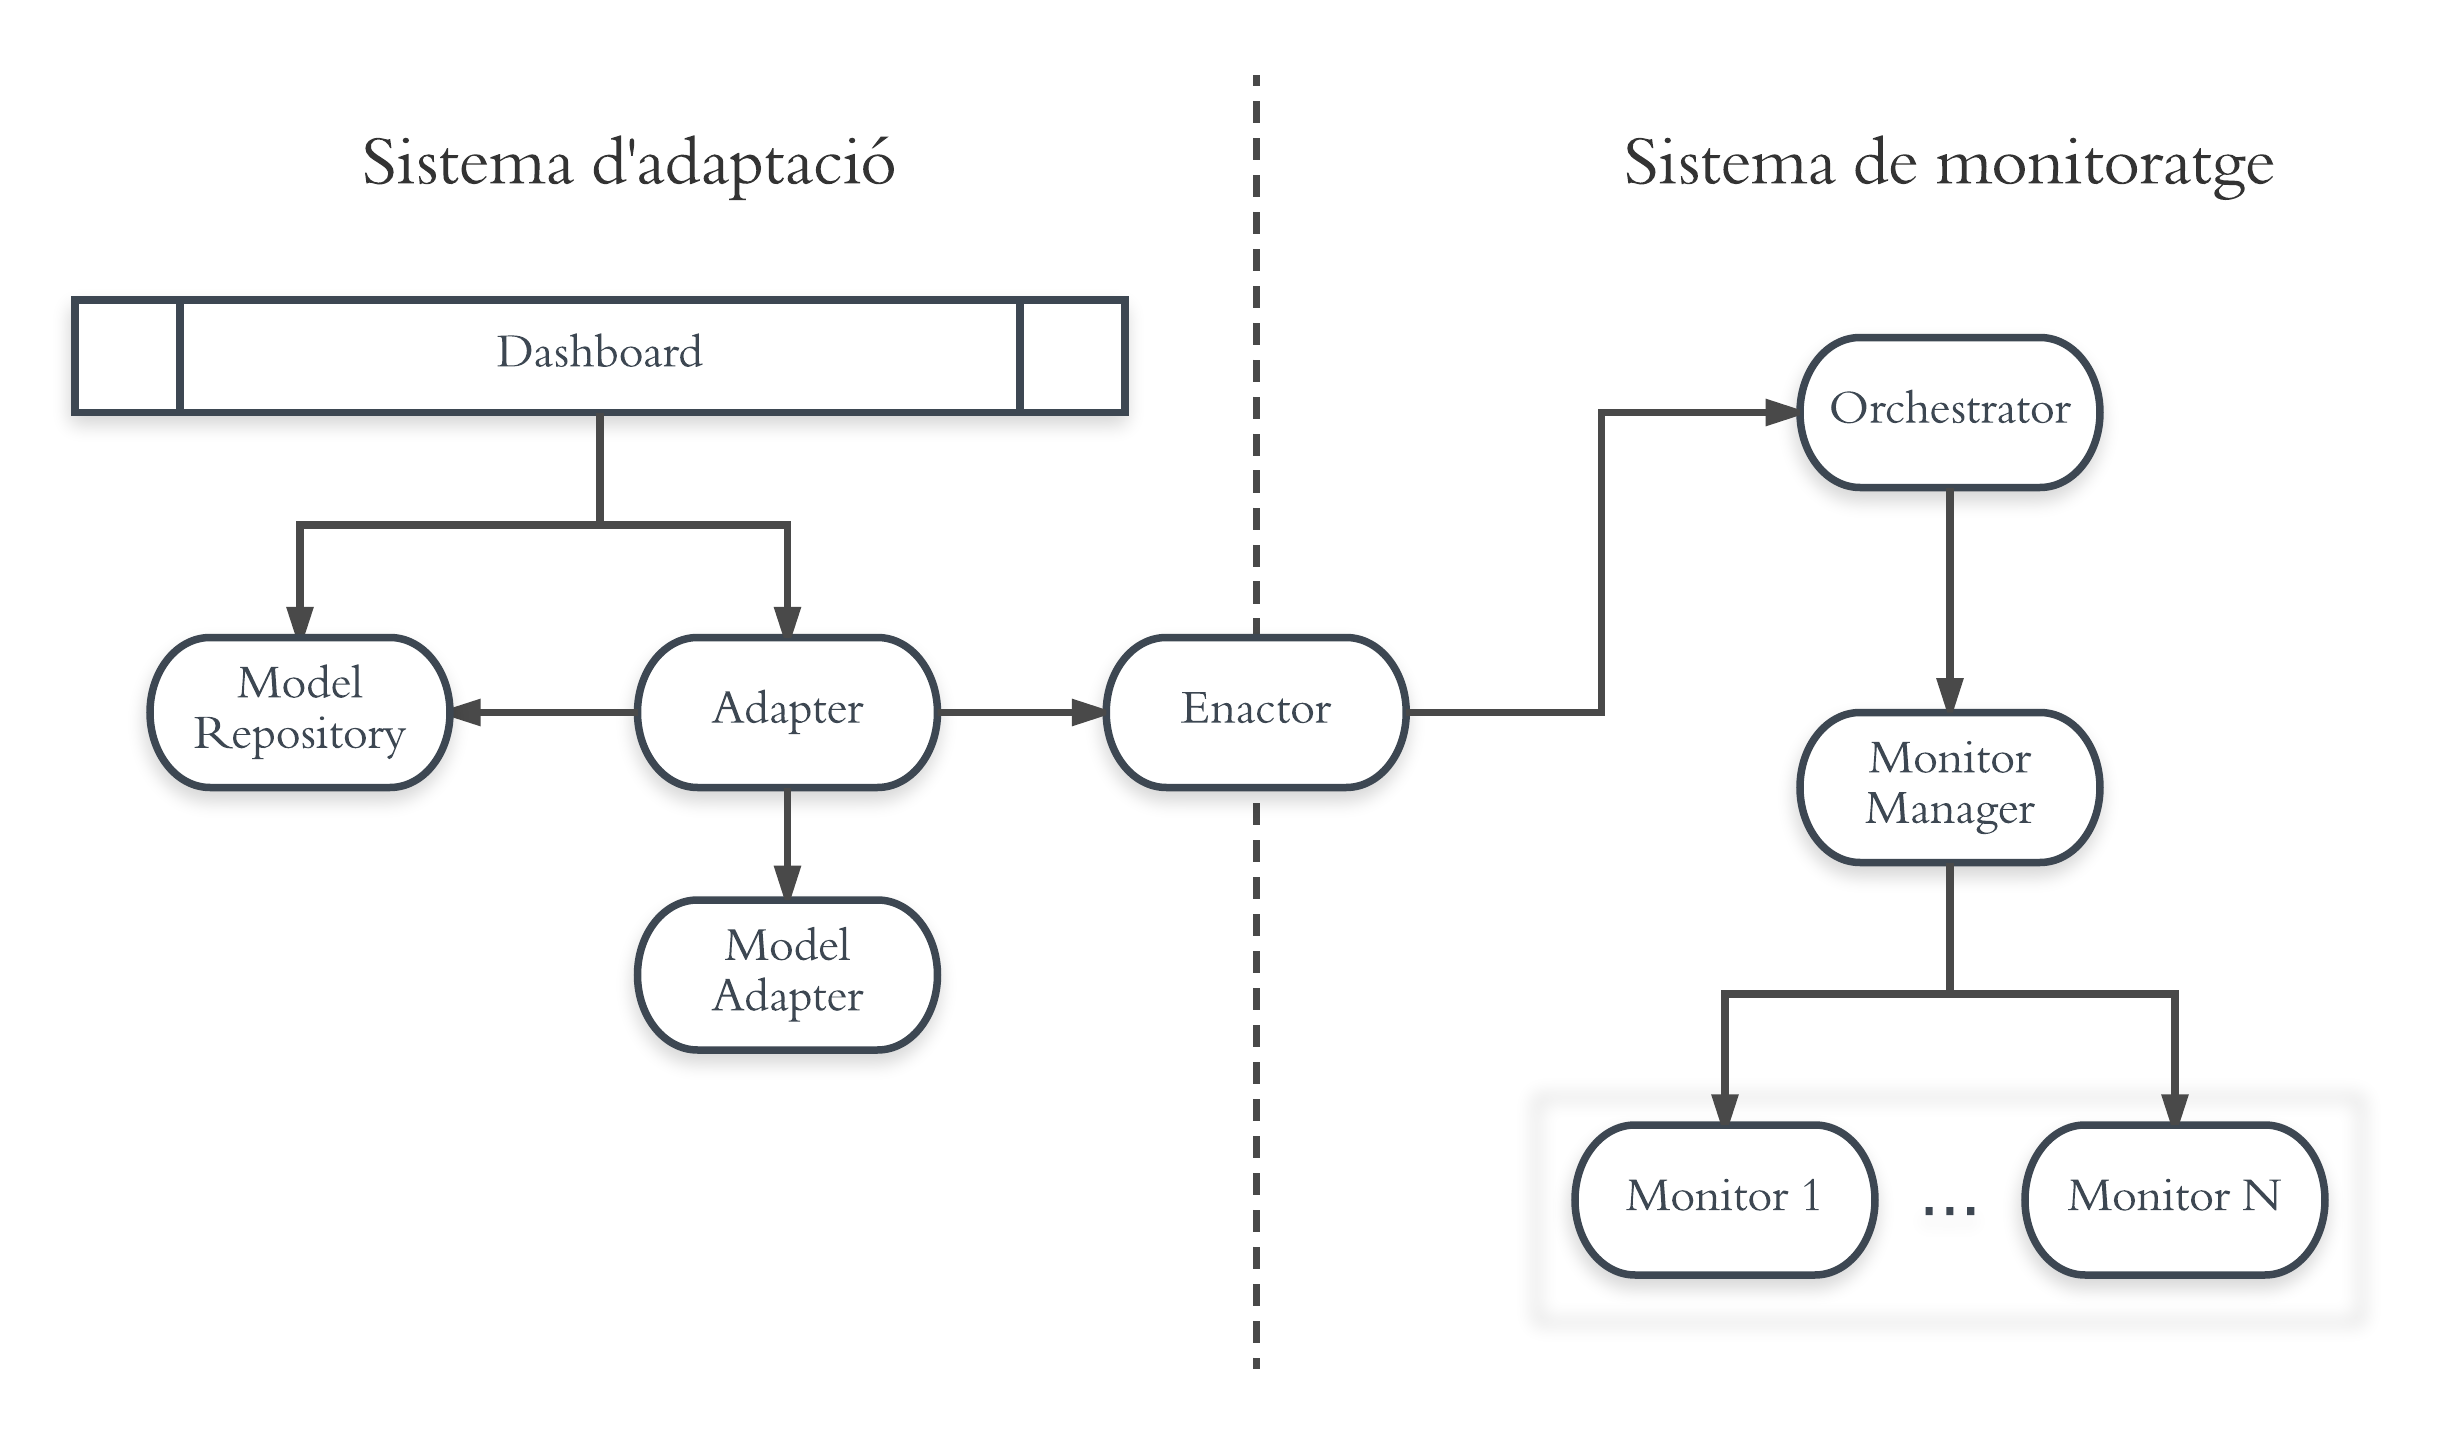
\includegraphics[width=13cm]{Figures/Figure4}
\decoRule
\caption[Disseny genèric del sistema proposat]{Disseny genèric del sistema proposat}
\label{fig:Figura4}
\end{figure}

\begin{itemize}
\item \textbf{Monitor.} Component de naturalesa ja descrita anteriorment, és l'encarregat de realitzar la col·lecció de dades d'un sistema software orientat al control de qualitat d'aquest. Dins el nostre sistema, disposarem d'un conjunt de monitors variats, conjunt que podrà ser extès sota diversos criteris i seguint el marc de la proposta de disseny plantejada.
\begin{itemize}
\item \textbf{\textit{Input}}. Informació/paràmetres de configuració d'un procés de monitoratge.
\item \textbf{\textit{Action}}. Procés de la informació per iniciar, aturar o modificar els paràmetres de la configuració d'un procés de monitoratge.
\item \textbf{\textit{Output}}. Conjunt de dades recol·lectades pels processos de monitoratge actius en el monitor.
\end{itemize}
\item \textbf{Monitor Manager.} Encarregat de gestionar l'activitat dels monitors, integrant el conjunt de monitors independents en el sistema sota un únic punt d'entrada, amb una semàntica genèrica. És l'encarregat, per tant, de redireccionar les diferents reconfiguracions (així com l'inici i aturada de processos de monitoratge) als monitors corresponents.
\begin{itemize}
\item \textbf{\textit{Input}}. Informació/paràmetres de configuració d'un procés de monitoratge per a un monitor específic.
\item \textbf{\textit{Action}}. Procés de la informació i transformació de la mateixa d'acord amb el monitor corresponent.
\item \textbf{\textit{Output}}. Informació/paràmetres de configuració transformats i orientats al monitor corresponent. 
\end{itemize}
\item \textbf{Orchestrator.} Aquest document forma part del context del projecte SUPERSEDE. Dins aquest projecte (presentat al capítol \textit{2.2.1. Projecte SUPERSEDE}), aquest component és el punt d'integració entre el subsistema d'adaptació de sistemes software i el subsistema de col·lecció i anàl·lisi de dades, i actua com a \textit{orquestrador} en un sentit de "pont" redireccional. En el marc del nostre projecte, que s'inclou a SUPERSEDE, aquest component actuarà com a punt entre el subsistema d'adaptació i el sistema de monitoratge
\begin{itemize}
\item \textbf{\textit{Input}}. Informació/paràmetres de configuració d'un procés de monitoratge per a un monitor específic.
\item \textbf{\textit{Action}}. Procés de la informació i transformació de la mateixa d'acord amb el propòsit del nostre sistema (configuració de monitors).
\item \textbf{\textit{Output}}. Informació/paràmetres de configuració transformats i orientats al sistema de monitoratge.
\end{itemize}
\end{itemize}

D'aquesta manera, el nostre sistema de monitoratge presenta 3 subcomponents independents que integren l'activitat de monitoratge mitjançant la comunicació entre ells: el sistema rep, a través de l'Orchestrator, peticions d'accions sobre els processos de monitoratge dels monitors. Aquest Orchestrator processa aquesta petició, i la redirecciona al Monitor Manager, qui coneix i controla els diferents monitors que hi ha al nostre sistema. El Monitor Manager s'encarrega d'analitzar la informació, processar-la d'acord al monitor al qual s'ha de redireccionar, i finalment enviar l'ordre de configuració al monitor corresponent. Amb aquesta informació ja processada per tal que el monitor concret pugui entendre-la, aquest adapta (és a dir, reconfigura) un procés de monitoratge existent, o bé en crea un de nou o n'elimina un d'existent, i procedeix amb el procés de monitoratge d'acord amb l'acció realitzada.\\

Definit els components del sistema de monitoratge, procedim a exposar els components i la interacció del \textbf{sistema d'adaptabilitat}:

\begin{itemize}
\item \textbf{Model Repository.} Aquest component s'encarrega de gestionar la persistència (lectura i escriptura) dels diferents models UML que defineixen les configuracions del nostre sistema de monitoratge. Els detalls d'aquests models UML, la seva sintaxi i el seu ús es descriuran més endavant.
\begin{itemize}
\item \textbf{\textit{Input}}. Peticions de lectura i escriptura dels models UML.
\item \textbf{\textit{Action}}. Accions pertinents sobre els models UML.
\item \textbf{\textit{Output}}. Retorna els models UML demanats d'acord amb la petició o modificació pertinent.
\end{itemize}
\item \textbf{Model Adapter.} Component que s'encarrega de realitzar adaptacions sobre els models UML que defineixen l'estat actual de les configuracions dels monitors d'acord amb les peticions d'adaptació que se li apliquen. Aquestes adaptacions sobre els diagrames definits s'apliquen en aquest component de forma aïllada, de manera que la resta del sistema no necessita tenir coneixement del procés tècnic de transformació dinàmica de models UML.
\begin{itemize}
\item \textbf{\textit{Input}}. Petició de modificació d'un model de configuració amb els models i paràmetres pertinents.
\item \textbf{\textit{Action}}. Modificació dinàmica del model UML d'acord amb la petició
\item \textbf{\textit{Output}}. Model UML transformat.
\end{itemize}
\item \textbf{Adapter.} És l'encarregat de realitzar l'adaptació del model des d'un punt de vista d'abstracció tècnica, centrant-se en la part semàntica de l'adaptació dels monitors. Mitjançant els models que defineixen el sistema i les possible millores, aquest component estudia i computa de forma automàtica reconfiguracions dels monitors.
\begin{itemize}
\item \textbf{\textit{Input}}. Lectura dels models del Model Repository per computar la petició d'adaptació de monitors.
\item \textbf{\textit{Action}}. Analitza els models i les possibles adaptacions per computar modificacions sobre els models de configuració, i demana aquesta modificació al Model Adapter.
\item \textbf{\textit{Output}}. Model/s de configuració adaptats.
\end{itemize}
\end{itemize}

En definitiva, el sistema d'adaptabilitat defineix un \textit{workflow} basat en una petició de reconfiguració a l'Adapter que, mitjançant l'anàl·lisi dels models que defineixen les configuracions dels monitors (configuracions actuals, suggerències de noves configuracions, etc.) computa una modificació real sobre la configuració actual.\\

En aquest punt, necessitem un últim component que actui de pont entre el sistema d'adaptabilitat i el sistema de monitoratge, de tal manera que les adaptacions realitzades en el sistema d'adaptabilitat sobre els models UML que defineixen l'estat del sistema de monitoratge s'apliquin a aquest darrer. En aquest sentit, s'introdueix el component \textbf{Enactor.}

\begin{itemize}
\item \textbf{Enactor.} Component d'integració entre les adaptacions generades pel sistema i el sistema de monitoratge. Concretament, actua de pont entre l'Adapter, encarregat de gestionar aquestes reconfiguracions, i l'Orchestrator, component del sistema genèric a SUPERSEDE encarregat de gestionar totes les peticions d'adaptabilitat de components software. La seva tasca principal és afegir una capa d'abstracció entre els dos subsistemes, per evitar que aquests hagin de conèixer de l'activitat de l'altre.
\begin{itemize}
\item \textbf{\textit{Input}}. Model UML adaptat generat per l'Adapter amb una nova proposta de configuració del sistema.
\item \textbf{\textit{Action}}. Transformació del model UML en format processable per l'Orchestrator.
\item \textbf{\textit{Output}}. Petició de reconfiguració d'un monitor específic que envia a l'Orchestrator.
\end{itemize}
\end{itemize}

A termes genèrics, i sense entrar encara en detalls de disseny intern de cadascun d'aquests components, tenim una proposta inicial genèrica que defineix com ha de ser el nostre sistema, quins components l'han de formar i com s'han de relacionar entre ells per satisfer l'objectiu genèric d'aquest projecte.\\

Com a punt addicional, es proposa també el disseny d'un \textbf{dashboard} basat en un aplicatiu web senzill, a través del qual poguem visualitzar algunes de les dades de les adaptacions generades pel nostre sistema, amb l'objectiu de facilitar el control de l'activitat del sistema i la validació del mateix per una possible demostració.

\section{Integració de components}

La interacció entre els diferents components del sistema haurà de ser un dels elements a tractar en el desenvolupament del projecte. Un dels objectius principals és garantir el màxim desacoblament entre cadascuna d'aquestes interaccions, de tal manera que cadascun dels components puguin ser reaprofitats de forma independement, i que a més la major part de modificacions en aquests components no afectin a la resta, com a mínim en termes d'interacció.\\

Per facilitar aquesta integració, el projecte SUPERSEDE ofereix una plataforma anomenada \textit{Integrated Framework} (IF), desenvolupada per un partner del projecte. El seu objectiu és oferir una integració de tots els components desplegats al \textit{back-end} del sistema. A nivell tècnic, aquest component ofereix una llibreria amb un conjunt de \textit{proxies} implementats, a través dels quals els diferents components es poden comunicar amb altres components desplegats i afegits al IF.\\

Per permetre aquesta integració, l'únic requisit que planteja aquesta plataforma és l'exposició dels diferents components com a serveis web RESTful. D'aquesta manera, IF actua com a pont directe sense necessitat de formatar o mapejar els paràmetres d'entrada i sortida d'aquestes interaccions, ja que aquest component s'encarrega de fer les transformacions pertinents d'acord amb les necessitats d'interacció. \\

Veurem més endavant com aquest sistema aprofita aquest framework per facilitar la comunicació i evitar mapejats d'entrada/sortida. Amb aquest objectiu, serà necessari exposar alguns dels components com a serveis web.
% Chapter Template

\chapter{Entorn de desenvolupament} % Main chapter title

\label{EinesDesenvolupament} % Change X to a consecutive number; for referencing this chapter elsewhere, use \ref{ChapterX}

El desenvolupament del sistema proposat requereix la integració d'un conjunt de subcomponents independents que, tot i comunicar-se entre ells, presenten una sèrie de característiques tècniques variades. Els requisits de desenvolupament i els entorns sobre els quals aquests components s'han de desenvolupar dependran de la naturalesa i els objectius de cadascun d'aquests. I, en termes genèrics, la gestió del sistema requerirà l'ús d'eines que ens facilitin aquest comportament.\\

Com a punt de partida al desenvolupament i exposició dels diversos components i tecnologies utilitzades, plantegem les tecnologies i elements bàsics que formen part del desenvolupament del projecte per, a partir d'aquí i al llarg dels següents capítols, exposar les tecnologies (llibreries, frameworks, etc.) que integrarem a aquestes per assolir els objectius.

\section{Tecnologies utilitzades}

Procedim a identificar les tecnologies bàsiques, amb les seves versions corresponents:

\begin{itemize}
\item \textbf{Git / GitHub (http://github.com).} Com a software de control de gestions i repositori s'utilitza \textbf{git} i \textbf{GitHub}, respectivament. La completesa i maduresa de git en la seva actualitat, així com les funcionalitats oferides per GitHub i la comoditat de la seva gestió, les fan candidates ideals per a realitzar el desenvolupament del projecte.
\item \textbf{Java 8.} Pràcticament la totalitat del projecte i els seus components s'han implementat utilitzant llenguatge Java. Concretament, la darrera versió Java 8, degut a les millores i la correcció d'alguns bugs que suposa respecte la seva anterior versió, Java 7.
\item \textbf{Eclipse IDE for Java Developers (Neon 4.6.2).} IDE i versió corresponents utilitzats pel desenvolupament dels components. S'ha considerat com l'opció ideal per una banda, per facilitar la compatibilitat i integració amb el projecte SUPERSEDE i els altres components, i per altra banda per la senzillesa i la integració de diferents plug-ins i eines que faciliten el desenvolupament. 
\item \textbf{Eclipse Modeling Tools (Neon 4.6.2).}  IDE complementari al desenvolupament orientat al desenvolupament de projectes de creació i edició de models UML mitjançant l'ús de tecnologies associades que es detallaran més endavant. 
\item \textbf{Gradle 2.13.} Davant la necessitat de gestionar les dependències i la compilació dels diferents components, s'ha triat Gradle com a opció preferent.
\item \textbf{Spring Framework 4.3.9.} Framework popularment conegut orientat al desenvolupament d'aplicacions basades en Java. L'utilitzarem especialment orientat a:
\begin{itemize}
\item Disseny i implementació de serveis web RESTful
\item Desenvolupament d'aplicacions web senzilles
\item Gestió de persistència d'aplicacions
\end{itemize}
\item \textbf{UML2 5.0.0.} Llibreria que encapsula la implementació per la gestió dinàmica mitjançant la plataforma Eclipse de models UML. L'utilitzarem per la lectura i escriptura dels models del nostre sistema de monitoratge.
\item \textbf{Papyrus 2.0.2.} Framework que ofereix un entorn de modelació gràfic dels models UML, els seus components i les seves propietats. Especialment útil per la visualització de models i el seu tractament per facilitat la seva lectura i anàlisi.
\end{itemize}

\section{Implementació i artefactes generats}
% Chapter Template

\chapter{Sistema de monitoratge} % Main chapter title

\label{SistemaMonitoratge} % Change X to a consecutive number; for referencing this chapter elsewhere, use \ref{ChapterX}

En aquest punt tenim la base necessària per procedir a exposar el treball realitzat des d'un punt de vista de disseny software i implementació dels diferents components. Agafant com a referència la solució proposada al \textit{Capítol 5. Visió general del sistema}, procedirem a desenvolupar els detalls tècnics de cadascun dels components que integren aquest sistema. Començarem per explicar els detalls relacionats amb el disseny i la implementació dels monitors.

\section{Monitors}

Recordem que, dins el nostre context, un \textbf{monitor} consisteix en un \textbf{component software} autònom amb una activitat regular orientada al control de qualitat d'un altre sistema software. Aquest control de qualitat es basa en una col·lecció de dades obtingudes a través d'aquest segon sistema, que ens aporten informació pròpia del context monitorat. Amb aquestes dades, un sistema capacitat per processar i analitzar aquestes dades, es poden generar suggerències de modificacions. Aquesta darrera part, però, queda fora de l'abast del nostre projecte, que centrarà l'activitat dels monitors en la seva tasca principal: la col·lecció de dades sota una sèrie de criteris específics.\\

En general, per tant, volem que el nostre sistema disposi d'un conjunt de monitors heterogenis (i, per tant, de naturalesa i comportament diferents), que puguin ser capaços de gestionar \textbf{processos de monitoratge} de forma paral·lela. És a dir: cadascun d'aquests monitors ha de ser capaç d'inicialitzar processos de monitoratge que s'executin en paral·lel i en segon pla, col·lectin dades d'acord als criteris de cadascun d'aquests processos, i les redireccionin a un tercer component software, encarregat del seu anàlisi.Per tant, necessitem que cadascun d'aquests monitors satisfaci els següents requisits funcionals:

\begin{enumerate}
\item \textbf{Inicialització de procés de monitoratge.} El monitor ha de poder rebre una petició per inicialitzar un nou procés de monitoratge amb una sèrie de paràmetres de configuració que defineixin aquest procés de monitoratge.
\item \textbf{Modificació de procés de monitoratge.} Donat un procés de monitoratge ja existent, el sistema ha de permetre la seva reconfiguració. És a dir: el sistema ha de permetre modificar els paràmetres d'aquest procés i, en conseqüència, alterar el comportament del procés (d'acord amb els criteris que es presenten a continuació.
\item \textbf{Aturada de procés de monitoratge.} Donat un procés de monitoratge ja existent, el sistema ha de permetre la seva aturada. Davant aquesta petició, el procés s'atura, i per tant es deixen de recol·lectar dades sota aquells criteris de monitoratge.
\end{enumerate}

\subsection{Especificacions tècniques}

Tal i com establiem com a objectiu principal del projecte, aquest sistema de monitoratge ha de ser \textbf{heterogeni}. La conseqüència principal d'aquesta característica és que necessitem definir un sistema que contempli que cadascun d'aquests requisits funcionals es garanteixen en la integració dels monitors implementats, i que per tant esdevenen casos d'ús complets i satisfactoris del nostre context. Per fer-ho, i donat que els monitors seran el principal punt de variabilitat del nostre sistema, hem d'afegir un cert nivell d'abstracció, un \textbf{desacoblament} entre els detalls específics de cadascun dels monitors, que ens resulten indiferents per la resta del sistema.\\

Per tant, el primer pas que hem de realitzar és \textbf{dissenyar una arquitectura} i uns \textbf{criteris de configuració genèrics} que satisfacin dos criteris: primerament, que ens permetin integrar tots els monitors implementats sota aquesta proposta al nostre sistema; i en segon lloc, que permetin una independència suficient com per garantir el criteri d'heterogeneïtat dels monitors. Desenvoluparem aquesta proposta analitzant els següents punts:

\begin{enumerate}
\item \textbf{Comportament intern del monitor.} Anàlisi de les necessitats i detalls tècnics del funcionament intern del procés de monitoratge.
\item \textbf{Redirecció de dades col·lectades.} Especificacions tècniques del mètode de gestió i redirecció de dades.
\item \textbf{Configuració dels monitors.} D'acord amb les necessitats anteriors, descriure quins paràmetres necessitarem per configurar els monitors.
\end{enumerate}

\subsubsection{Comportament intern del monitor}

La implementació d'un monitor representa, des d'un punt de vista semàntic, un component software encarregat de monitorar un component software concret. En aquest context específic, entendrem \textbf{monitorar} com la col·lecció periòdica d'un conjunt de dades produïdes de l'execució del sistema software monitorat. En base a aquesta definició, entendrem com a \textbf{procés de monitoratge} el cicle següent:

\begin{enumerate}
\item Inicialització de les estructures de col·lecció de dades
\item Captura de dades durant el transcurs d'un període de temps determinat
\item Enviament de les dades a un tercer component software
\end{enumerate}

Així, de forma periòdica, un procés de monitoratge recull durant un període de temps (o \textbf{\textit{time slot}}) específic totes les dades que el monitor ha estat configurat per recollir. Per tal que els monitors es puguin explotar al màxim, és imprescindible que aquests permetin l'\textbf{execució en paral·lel} de diversos processos de monitoratge, amb possibles diferències en els seus paràmetres de configuració (p.e., aquest \textit{time slot}).\\

Davant aquesta proposta, el comportament i potencial d'un monitor queda molt limitat, ja que elements com p.e. el mètode de recollida de dades, o fins i tot les dades recollides, queden molt limitats. En general, és molt possible que un sistema software pugui ser monitorat mitjançant diferents tècniques, com per exemple l'ús d'APIs, llibreries o components externs, etc. Per aquesta raó, si volem permetre que el nostre monitor ofereixi flexibilitat en aquest aspecte, hem de permetre l'ús de diferents eines, o \textbf{\textit{tools}}, que aquest monitor pot utilitzar indistintament per executar els processos de monitoratge.\\

La integració de diverses \textit{tools} dins un monitor ens permeten no només una variabilitat en l'execució de la col·lecció de dades, sinó també una major fiabilitat i qualitat del monitor com a component software. Ens permet reaccionar, entre d'altres, davant escenaris on l'ús d'un sistema de monitoratge específic deixa de funcionar (p.e. una API que no dona resposta), ja que davant la detecció d'aquest error el canvi de \textit{tool} utilitzada ens permet que el monitor no deixi de ser usable.\\

En resum, necessitem que el monitor sigui capaç de gestionar un nombre indefinit de processos de monitoratge en paral·lel, amb configuracions diferents, i que utilitzin el conjunt de \textit{tools} implementades.

\subsubsection{Redirecció de dades col·lectades}

Un dels objectius de les especificacions tècniques dels monitors és permetre la seva integració, en primer lloc, dins el context del nostre projecte, i en segon lloc, a sistemes tercers que permetin l'anàlisi de les dades recollides durant la seva activitat de monitoratge. D'aquesta manera augmentem el valor propi dels components dissenyats en el projecte, reutilitzable en contexts diferents al plantejat. Per aquesta raó, i per completar l'activitat del monitor, hem de contemplar com dissenyar l'enviament i redirecció de les dades que cada monitor recull i formata durant la seva activitat. \\

Per facilitar aquest aspecte, i permetre també la seva integració dins el sistema general de SUPERSEDE, els monitors integraran la implementació d'enviament de les seves dades a través d'\textbf{Apache Kafka.} Es tracta d'una plataforma distribuïda de \textit{streaming} que ofereix la possibilitat de crear i configurar \textit{pipelines} de dades en temps real que actuen com a canal de comunicació entre diverses aplicacions o components software. L'arquitectura és senzilla: un component software, anomenat \textbf{\textit{producer}}, es comunica amb el servidor Kafka i envia dades de forma periòdica a un \textit{pipeline} específic d'aquest servidor, prèviament configurat i identificament amb el que anomenem Kafka \textit{topic}, un identificador únic d'aquell \textit{pipeline} per aquell desplegament de Kafka. Aquest flux de dades s'encua al servidor, i es redireccionen a uns altres sistemes o aplicacions, anomenats \textbf{\textit{consumers}}, que reben i processen les dades d'un pipeline específic a mesura que es van enviant i processant.\\

\begin{figure}
\centering
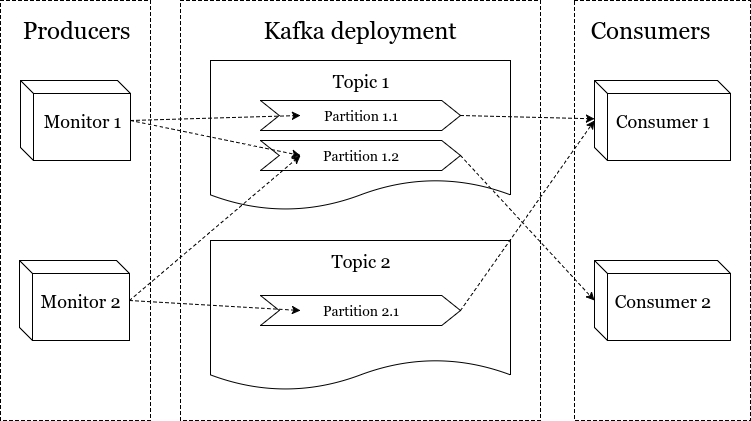
\includegraphics[width=11cm]{Figures/Figure7}
\decoRule
\caption[Exemple d'arquitectura de la comunicació amb Kafka]{Exemple d'arquitectura de la comunicació amb Kafka}
\label{fig:Kafka}
\end{figure}

En general, l'avantatge principal de Kafka i la justificació del seu ús pel nostre context és que permet una integració còmode i fiable entre diferents aplicacions que necessiten comunicar dades de forma periòdica, garantint la seva arribada. Kafka ofereix una sèrie d'APIs per configurar els \textit{producers} i \textit{consumers}, així com una configuració relativament senzilla del propi servidor. Gràcies a aquestes característiques, podem aprofitar els propis monitors per actuar com a \textit{producers} d'un \textit{stream} de dades, que es correspondrà amb les dades monitorades durant els processos d'execució, i distribuïr-les als diferents \textit{pipelines} o Kafka \textit{topics}. Així, davant possibles ampliacions i expansions d'aquest projecte, podem fàcilment incorporar components d'anàlisi gràcies al desacoblament entre la lògica interna del monitor i l'enviament i captura de dades que l'arquitectura de Kafka ens ofereix.\\

La lògica interna genèrica proposada per la implementació dels monitors serà, per tant, l'ús de l'API de \textit{producer} de Kafka per part dels monitors, pel qual cada procés de monitoratge enviarà de forma periòdica dades a un servidor Kafka específic, o Kafka \textit{endpoint}, i dins aquest desplegament, a un \textit{pipeline} o Kafka \textit{topic} específic. A la figura ~\ref{fig:Kafka} s'exposa com funciona aquesta comunicació entre els monitors i els \textit{consumers}, components que poden ser de qualsevol tipus sempre i quant implementin la lògica de \textit{consumers} pròpia e Kafka.

\subsubsection{Paràmetres de configuració}

Davant les especificacions anteriors, i per garantir el màxim nivell de personalització i configuració dels monitors, cadascun dels processos de monitoratge actius en un monitor ha de permetre definir els paràmetres relacionats amb les possibles variacions i diferències entre aquests processos, tant en temps de creació com durant la seva reconfiguració. En aquest sentit, es proposen els següents paràmetres com a genèrics per a totes les implementacions de monitors:

\begin{itemize}
\item \textbf{\textit{Time slot}}. Expressat en segons, indica la durada de cada període de monitoratge de dades (és a dir, temps que transcorre cada vegada que s'envia un nou \textit{stream} de dades).
\item \textbf{\textit{Tool name}}. Nom de l'eina (\textit{tool}) utilitzada per aquell procés de monitoratge, i que per tant implica la col·lecció d'unes dades específiques utilitzant una tècnica específica.
\item \textbf{\textit{Kafka endpoint}}. Adreça que apunta al servidor on es troba desplegat el sistema Kafka on s'han d'enviar les dades generades, ja sigui \textit{localhost} o URL pública.
\item \textbf{\textit{Kafka topic}}. Identifica el \textit{pipeline} de dades del servidor Kafka on el monitor (\textit{producer} dins el context de Kafka) ha d'enviar les dades.
\end{itemize}

És possible, tal i com veurem més endavant, que alguns monitors requereixin de paràmetres de configuració addicionals, propis del funcionament intern específic del monitor. Per aquest motiu, a banda de proporcionar una configuració bàsica pels monitors amb els paràmetres anteriors, cal permetre també una extensibilitat en quant a paràmetres de configuració.

\subsection{Arquitectura genèrica}

\begin{figure}
\centering
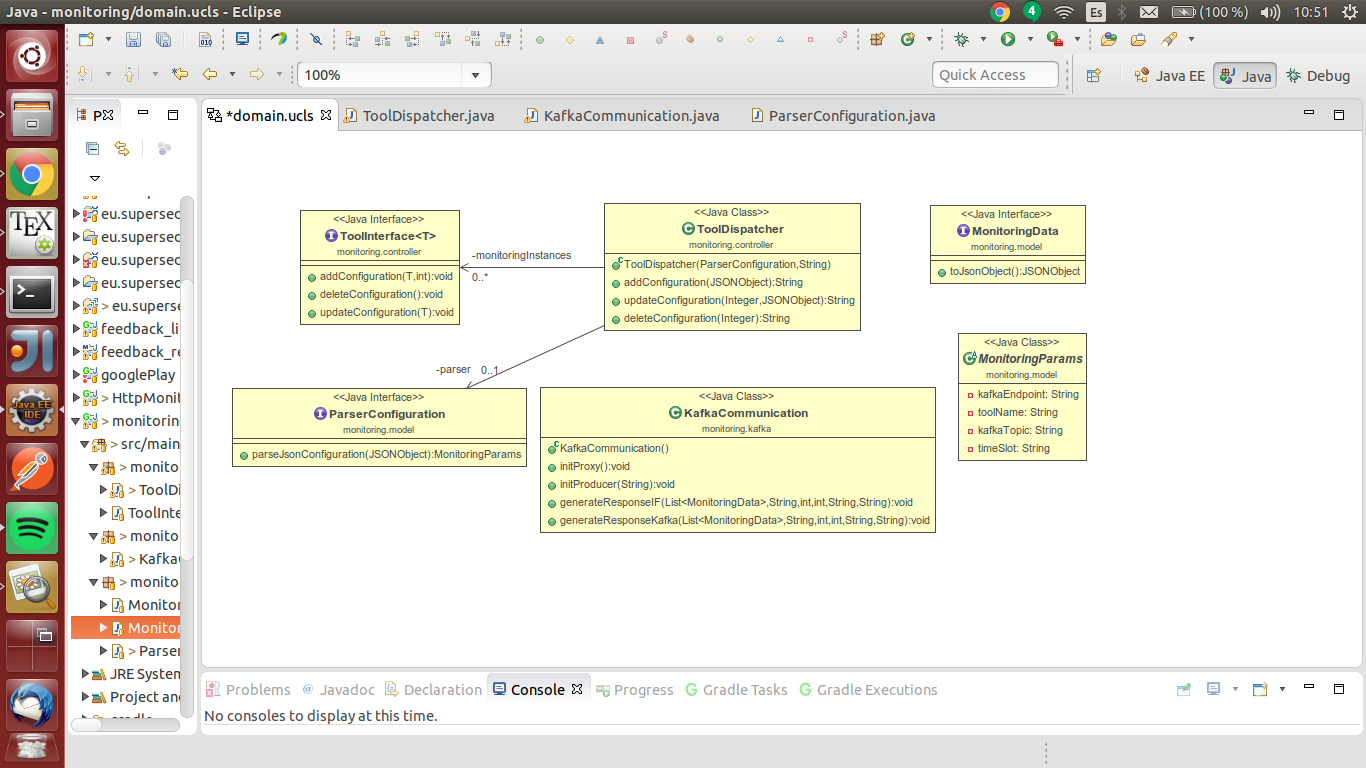
\includegraphics[width=14cm]{Figures/Figure5}
\decoRule
\caption[Arquitectura software genèrica d'un monitor]{Arquitectura software genèrica d'un monitor}
\label{fig:Figura5}
\end{figure}

Es proposa l'arquitectura definida a la figura ~\ref{fig:Figura5} a extendre per cadascuna de les implementacions de monitors. Per entendre aquesta arquitectura, a continuació s'expliquen cadascun dels elements integrats:

\begin{itemize}
\item \textbf{MonitoringParams}. Classe abstracta que cada monitor ha d'implementar que conté, de base, els paràmetres de configuració dels monitors genèrics per tots aquests. Addicionalment, cada implementació de monitor pot afegir els paràmetres i la lògica associada a aquests que consideri oportuns.
\item \textbf{ParserConfiguration}. Interfície que cada monitor ha d'implementar i que defineix un mètode per transformar un objecte JSON en una instància de la classe \textit{MonitoringParams} implementada pel propi monitor. L'objectiu és permetre així que el monitor pugui processar JSON com a format de comunicació estàndar per les peticions de configuracions, facilitant el seu ús desplegat com a servei web (especialment útil per l'Integrated Framework dins el context SUPERSEDE, tal i com s'explica al \textit{Capítol 5. Visió general del sistema}).
\item \textbf{ToolInterface}. Interfície parametritzada amb una especialització de la classe \textit{MonitoringParams} que defineix una instància de procés de monitoratge per una \textit{tool} específica. Defineix els següents mètodes:
\begin{itemize}
\item \textbf{\textit{addConfiguration(T)}} -> inicialitza el procés de monitoratge amb els paràmetres definits per la instància de T (subclasse de MonitoringParams)
\item \textbf{\textit{deleteConfiguration()}} -> atura el procés de monitoratge i elimina la instància de la \textit{tool}
\item \textbf{\textit{updateConfiguration(T)}} -> actualitza els paràmetres de configuració del procés iniciat en segon pla per la instància de la \textit{tool}
\end{itemize}
\item \textbf{ToolDispatcher}. Classe que actua com a controlador del monitor, rebent totes les peticions relacionades amb els processos de monitoratge i gestionant les diferents instàncies en execució. Defineix un \textit{ParserConfiguration} per processar la traducció de JSON (format estàndar) a \textit{MonitoringParams} pels següents mètodes:
\begin{itemize}
\item \textbf{\textit{addConfiguration(JSONObject)}} -> processa els paràmetres definits al JSONObject i inicialitza una instància de la \textit{tool} corresponent amb els paràmetres associats
\item \textbf{\textit{deleteConfiguration(int)}} -> atura el procés de monitoratge identificat per l'id proporcionat
\item \textbf{\textit{updateConfiguration(JSONObject, int)}} -> actualitza els paràmetres de configuració definits al JSONObject del procés de monitoratge identificat per int
\end{itemize}
Per tal de gestionar la \textit{tool} utilitzada en cada procés de monitoratge (que representarà una nova instància de la implementació de la interfície \textit{ToolInterface}) utilitzant el paràmetre \textit{toolName} de configuració, s'utilitza el patró \textit{reflection}. Aquest patró de disseny software es caracteritza per la modificació en temps d'execució del comportament d'un sistema; i, en el nostre cas, ens interessa per permetre  la instanciació de les diferents \textit{tools} utilitzant el seu nom sense necessitat de coneixe'l. Mitjançant l'ús del nom de la tool, i coneixent el \textit{package} on es troben implementades les tools, podem instanciar aquella tool partint únicament del nom, sense necessitat de cap altre tipus de context.
\item \textbf{MonitoringData}. Interfície que cada monitor implementa amb les dades i format que el monitor genera fruït de la seva activitat, amb la implementació d'un mètode \textit{toJsonObject()} per definir un format genèric de les dades a enviar
\item \textbf{KafkaCommunication}. Classe que implementa la comunicació amb el servidor de Kafka, i que permet enviar les dades generades per l'activitat de monitoratge. Implementa 4 mètodes segons les dues lògiques de comunicació possibles: la integrada al sistema SUPERSEDE (utilitzant \textit{proxies} de IF), i una configuració personalitzable a un Kafka endpoint específic:
\begin{itemize}
\item \textbf{\textit{initProxy()}} -> inicialitza la instància de \textit{proxy} que permet la comunicació amb el Kafka \textit{server} desplegat a IF
\item \textbf{\textit{generateResponseIF(List<MonitoringData>)}} -> envia el llistat d'instàncies de dades monitorades a través del \textit{proxy} inicialitzat
\item \textbf{\textit{initProducer(String)}} -> inicialitza un \textit{producer} de Kafka que es comunica amb l'\textit{endpoint} especificat
\item \textbf{\textit{generateResponseKafka(List<MonitoringData>)}} -> envia el llistat d'instàncies de dades monitorades a través del \textit{producer} inicialitzat
\end{itemize}
\end{itemize}

Aquesta és per tant la proposta d'una arquitectura genèrica per la implementació de cadascun dels monitors a integrar en el nostre sistema. Les especificacions tècniques tant des d'un punt de vista de requisits funcionals com requisits arquitectònics o de qualitat queden garantides, així com la seva extensibilitat d'acord amb les característiques específiques necessàries de cada monitor. La proposta genèrica s'implementa en un projecte del qual les implementacions de monitors específics han d'estendre com a subprojecte, utilitzant les funcionalitats de Gradle a tal efecte.

\subsection{Implementació de monitors}

Un cop exposada l'arquitectura i especificacions genèriques dels monitors, el següent pas és procedir a la implementació dels diferents monitors que integrarem al nostre sistema. Aquestes implementacions esdevindran possibles casos d'ús a executar, però únicament suposen exemples dins d'un ample ventall de possibilitats d'implementació.\\

En aquest projecte presentem la implementació de 3 monitors classificats en 2 tipus de monitors diferents: \textbf{monitors de xarxes socials} i \textbf{monitors de botigues d'aplicacions}. Pel primer tipus, es proposa un monitor de la xarxa social \textbf{Twitter}. Pel segon tipus, es proposen dos monitors: un monitor de \textbf{Google Play} i un altre de l'\textbf{App Store}. 

\subsubsection{Twitter Monitor}

L'objectiu d'aquest monitor és supervisar i recol·lectar els tuits publicats a la xarxa social de Twitter durant un període de temps concret (definit al procés de monitoratge) que compleixen una sèrie de característiques específiques, d'acord amb els criteris que poden resultar d'interès en quant a la informació d'aquests tuits. \\

Per permetre aquesta activitat de monitoratge, i tal i com procedirem amb cadascun dels monitors, necessitem implementar com a mínim una \textit{tool} amb la qual realitzar el procés de monitoratge. Definirem una \textit{tool} anomenada \textbf{TwitterAPI} que utilitzarà \textbf{twitter4j}, una llibreria lliure no oficial de Java que permet utilitzar una arquitectura ja definida per connectar-se a les APIs de Twitter, i entre d'altres a la \textbf{Stream API}, una API que permet obrir \textit{streams} de dades per capturar i processar tots els tuits publicats en temps real que compleixin una sèrie de característiques específiques. Aquests \textit{streams} s'executaran com a \textit{threads} en segon pla i en paral·lel d'acord amb el nº de processos de monitoratge oberts.\\

Pel nostre cas, definirem dos paràmetres per filtrar els tuits monitorats: l'\textbf{autor} del tuit i l'aparició d'un \textbf{conjunt de paraules} específic al contingut del tuit. Per configurar cadascun dels processos de monitoratge d'acord a aquests dos criteris, caldrà afegir els següents paràmetres:

\begin{itemize}
\item \textbf{accounts} - llistat amb els identificadors dels autors dels quals volem obtenir els tuits 
\item \textbf{keywordExpression} - expressió booleana formada per combinacions AND, OR i NOT de diferents \textit{keywords} que el contingut del tuit ha de satisfer per ser monitorat
\end{itemize}

La \textit{Stream API} ofereix paràmetres de configuració per realitzar el \textit{tracking} dels tuits que satisfan ambdues condicions. En el cas del primer paràmetre \textit{accounts} no cal realitzar cap transformació, ja que únicament necessitem els noms únics de les comptes dels autors per obtenir els seus tuits. Contràriament, l'API únicament ofereix l'oportunitat de filtrar per combinacions de paraules expressades en la seva \textit{forma normal disjuntiva}, o \textbf{FND}. És a dir, expressions del format:\\

\centerline{\textit{$X_{1} \,\, OR \,\, X_{2} \,\, OR \,\, .. \,\, OR \,\, X_{n}$}}\bigskip

\noindent
on $X_{n}$ és una expressió booleana formada per una combinació indefinida d'operands AND:\\

\centerline{\textit{$keyword_{1} \,\, AND \,\, keyword_{2} \,\, AND \,\, .. \,\, AND \,\, keyword_{n}$}}\bigskip

Davant aquest fet, i per evitar forçar un format específic del paràmetre de configuració d'entrada, necessitem implementar una lògica interna pròpia de la \textit{tool} TwitterAPI que transformi qualsevol expressió booleana en la seva expressió FND. \\

\begin{figure}
\centering
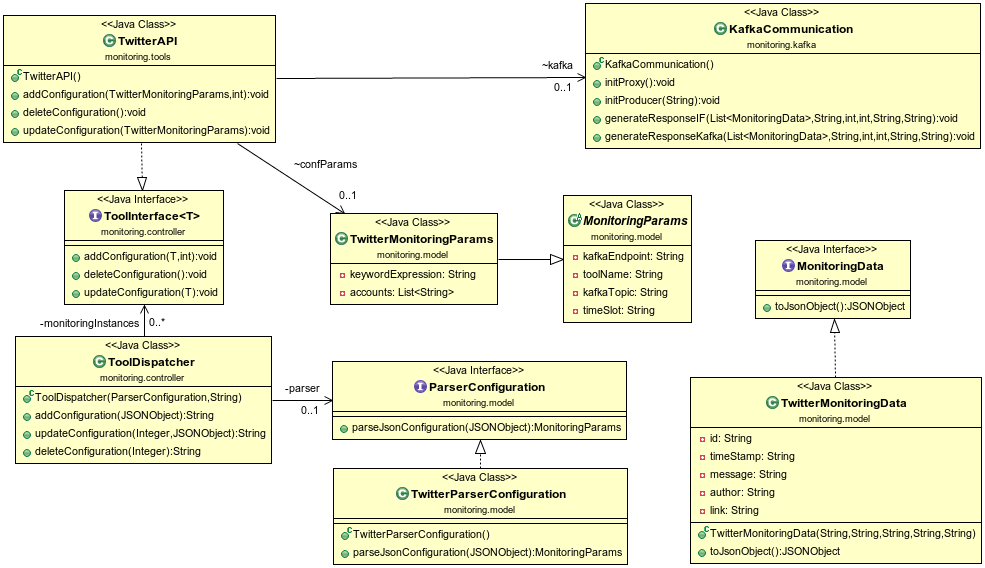
\includegraphics[width=14cm]{Figures/Figure6}
\decoRule
\caption[Arquitectura software del monitor de Twitter]{Arquitectura software del monitor de Twitter}
\label{fig:Figura6}
\end{figure}

Donats aquests detalls podem utilitzar l'arquitectura genèrica proposada anteriorment per extendre la implementació del monitor de Twitter. Aquesta arquitectura i els components implementats es troben definits a la figura ~\ref{fig:Figura6}, on podem veure aquells components reutilitzats de l'arquitectura genèrica remarcats en groc, per poder fer una comparativa ràpida sobre les classes i components que ha calgut implementar per poder definir un monitor:

\begin{itemize}
\item \textbf{TwitterMonitoringParams.} Subclasse de la classe abstracta \textit{MonitoringParams} que hereta per una banda els atributs comuns a tots els monitors (\textit{kafkaEndpoint, toolName, kafkaTopic} i \textit{timeSlot}) i per altra banda en defineix dos nous: la \textit{keywordExpression} i un llistat d'\textit{accounts}.
\item \textbf{TwitterParserConfiguration.} Implementació de la interfície que defineix la transformació del format d'entrada del monitor (JSONObject) a la instància de \textit{TwitterMonitoringParams} amb la qual el monitor (i en conseqüència la seva \textit{tool}) treballarà.
\item \textbf{TwitterMonitoringData.} Implementació de la interfície que defineix la transformació de les dades recollides durant un cicle del procés de monitoratge d'una \textit{tool} al format de sortida del monitor (JSONObject).
\item \textbf{TwitterAPI.} Implementació de la interfície que defineix la lògica de les tres operacions de qualsevol \textit{tool}: iniciar una nova configuració, modificar-ne una d'existent, i eliminar-ne una d'existent. En aquest cas disposem d'una única implementació, però tal i com veurem més endavant, l'arquitectura permet sense problema generar un conjunt de \textit{tools} diferenciades, cadascuna amb les seves característiques i dades internes, que utilitzaran les mateixes implementacions de formats de dades definides anteriorment. Aquest component serà l'encarregat d'utilitzar \textit{twitter4j} per configurar la crida a la Stream API i obrir el \textit{thread} encarregat d'anar rebent i emmagatzemant els tuits rebut. Addicionalment, serà també responsabilitat d'aquesta tool comunicar-se amb \textit{KafkaCommunication} per utilitzar el mètode de comunicació (a través de IF o personalitzat) que correspongui, d'acord amb les necessitats de la \textit{tool}.
\end{itemize}

A la figura \ref{fig:Figura12} es pot observar un exemple de l'objecte JSON generat a partir de la transformació definida per la implementació de la interfície \textit{MonitoringData}. Aquest objecte serà enviat, a través de la \textit{tool} i utilitzant la classe \textit{KafkaCommunication}, al Kafka \textit{endpoint} i Kafka \textit{topic} definits a la configuració del monitoratge. De les dades generades per la comunicació amb l'API, recollirem: \textit{idItem} (identificador del tuit), \textit{timeStamp} (moment en que s'ha realitzat el tuit), \textit{message} (contingut del mateix), \textit{author} (l'identificador de l'autor), i \textit{link} (enllaç al tuit a la plataforma Twitter). 

\begin{figure}[!h]
\centering
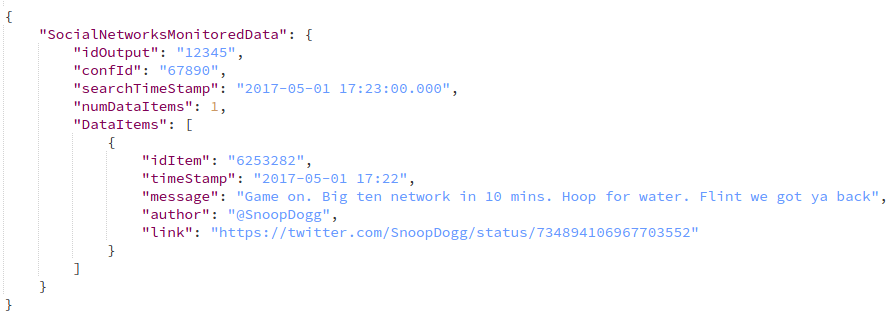
\includegraphics[width=14cm]{Figures/Figure12}
\decoRule
\caption[Exemple dades de sortida generades pel monitor de Twitter]{Exemple dades de sortida generades pel monitor de Twitter}
\label{fig:Figura12}
\end{figure}

Cal destacar que gràcies al disseny de l'arquitectura proposada anteriorment per la implementació d'un monitor integrat al nostre sistema (o, de fet, sense necessitat que l'objectiu final sigui la seva integració) ha requerit una extensió relativament senzilla. Únicament ha calgut implementar aquells aspectes propis de cada monitor, que en són 4: els paràmetres específics de configuració (1), el mapejat dels paràmetres d'entrada (2), el mapejat de les dades de sortida (3), i el funcionament de les \textit{tools} (en aquest cas, twitter4j) per realitzar els processos de monitoratge (4). D'aquesta manera satisfem un dels principals objectius: dotar al nostre sistema de la màxima extensibilitat i heterogeneïtat possible, amb la possibilitat de personalitzar l'activitat i semàntica de cada monitor partint d'una arquitectura comuna. \\

\noindent{\large{\textbf{Exposició com a servei REST}}}\\

El següent pas d'acord amb les necessitats tècniques per la integració és exposar el monitor i les seves funcionalitats com un servei web RESTful. D'aquesta manera, mitjançant la documentació d'una API per accedir a les diferents operacions d'alta, baixa i modificació d'un procés de monitoratge, podem integrar els monitors al IF del projecte SUPERSEDE i permetre així el seu accés a través de la plataforma d'integració. En aquest sentit l'ús de JSON com a format de comunicació d'entrada i sortida ens facilita la seva exposició com a servei web, que utilitzarà també el format JSON com a \textit{payload} per fer les crides. La documentació de l'API del monitor de Twitter es pot trobar a l'apèndix ~\ref{AppendixA}, on podem trobar en detall les peticions REST implementades, així com el format dels \textit{inputs} i \textit{outputs} de cadascuna de les crides.\\

Per tal de poder concebre com funcionaria la comunicació amb el monitor per iniciar una nova instància de monitoratge, la figura ~\ref{fig:Figura8} mostra un exemple d'objecte JSON utilitzat.

\begin{figure}[!h]
\centering
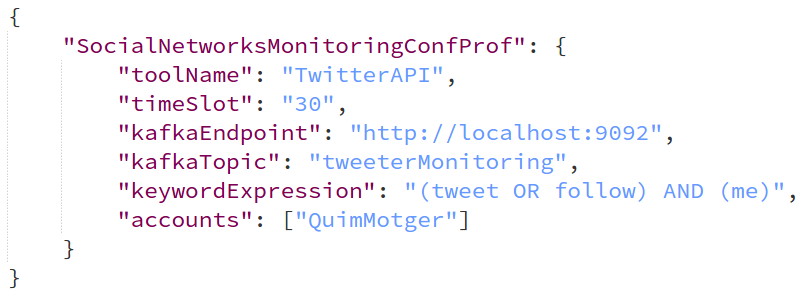
\includegraphics[width=11cm]{Figures/Figure8}
\decoRule
\caption[Exemple JSON de configuració del monitor de Twitter]{Exemple JSON de configuració del monitor de Twitter}
\label{fig:Figura8}
\end{figure}

En referència a aquesta possible petició, la figura ~\ref{fig:Figura9} mostra un exemple de la resposta (en cas d'èxit en la configuració del monitor) que retorna aquest monitor per la petició anterior. En aquesta figura, definim 2 paràmetres de retorn. Primerament,  \texttt{idConf}, que conté l'identificador de la nova instància de monitoratge creada (variable indispensable per tal que sigui usable i poder realitzar adaptacions posteriors). En segon lloc \texttt{status}, que indica si la petició s'ha realitzat amb èxit o s'ha produït algun error.

\begin{figure}[!h]
\centering
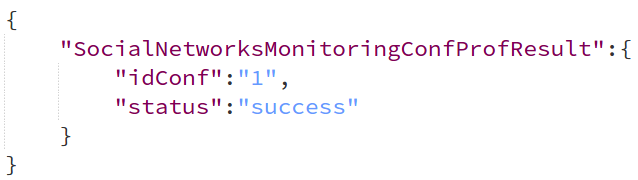
\includegraphics[width=8cm]{Figures/Figure9}
\decoRule
\caption[Exemple resposta amb èxit del monitor de Twitter]{Exemple amb èxit del monitor de Twitter}
\label{fig:Figura9}
\end{figure}

Donat el cas que s'hagi produït algun error, el format de resposta anterior no és vàlid (no s'ha creat cap instància i, per tant, cap identificador pot ser produït) ni suficient (no ens aporta informació de quin ha estat l'error). En aquest cas, un exemple de resposta seria l'exposat a la figura ~\ref{fig:Figura10}.

\begin{figure}[!h]
\centering
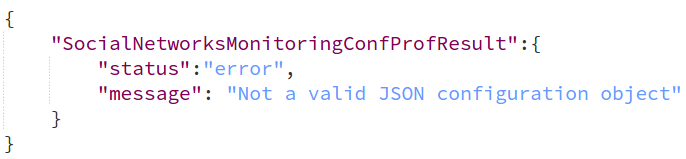
\includegraphics[width=10cm]{Figures/Figure10}
\decoRule
\caption[Exemple resposta amb error del monitor de  Twitter]{Exemple resposta amb error del monitor de Twitter}
\label{fig:Figura10}
\end{figure}

\subsubsection{Google Play Monitor}

Aquest segon monitor, encarregat del monitoratge de dades de la botiga d'aplicacions dels sistemes operatius Android, \textbf{Google Play}, pretén recollir les dades referents a les crítiques o \textit{reviews} que els usuaris de Google Play fan de les aplicacions que es descarreguen. De manera semblant al monitor de Twitter, però en un context i amb un objectiu diferent, recull dades dels usuaris i els missatges que publiquen al voltant d'un focus específic.\\

En aquest cas, i aprofitant que tenim definit un cas d'ús simple d'un monitor amb una sola \textit{tool}, podem procedir a explotar l'arquitectura dels nostres monitors i definir un monitor que utilitzi més d'una \textit{tool} per realitzar els processos de monitoratge. En aquest cas, s'ha fet una recerca a la xarxa sobre els diversos sistemes i components que existeixen (d'ús total o parcialment lliure) per realitzar el monitoratge, i s'han triat els dos següents degut a les seves característiques:

\begin{itemize}
\item \textbf{GooglePlayAPI}. \textit{Tool} que implementa una comunicació en 2n pla, similar al sistema de \textit{threads} emprat pel monitor de Twitter, amb la Google Play Developer API. Diem "similar" degut al fet que aquesta API, que funciona mitjançant un sistema d'autenticació OAuth 2.0, no permet obrir un \textit{stream} de dades com es presentava amb el monitor de Twitter, sino que permet obtenir, mitjançant crides API, les dades referents al conjunt total de \textit{reviews} publicades per una aplicació determinada en el moment de la crida. D'aquesta manera no podem obtenir un \textit{stream} de dades real de forma directa, sino que serà responsabilitat de la pròpia \textit{tool} simular aquest \textit{stream} de dades. Per fer-ho, realitzarem de forma periòdica (segons el \textit{timeSlot} definit) crides a l'API per obtenir aquestes dades, i la \textit{tool} s'encarregarà de recollir i retornar únicament les \textit{reviews} realitzades durant el període de monitoratge. Com a avantatge principal, aquesta \textit{tool} permet fer \textbf{fins a 60 crides} en 1 hora, un nombre molt elevat especialment si ho contrastem amb altres eines. Per contra, com a limitació únicament permet obtenir dades d'aplicacions de les quals l'usuari que s'ha autenticat n'és el propietari.
\item \textbf{GooglePlay-AppTweak}. Aquesta eina permet obtenir als usuaris registrats un ample ventall de dades de les aplicacions publicades a GooglePlay. En aquest cas, l'autenticació està basada en crides amb \textit{token}, i el sistema és similar a la \textit{tool} de GooglePlayAPI: necessitem simular dins el comportament de la mateixa \textit{tool} un \textit{stream} de dades parsejant els resultats de la consulta de les \textit{reviews} públiques fins al moment de la crida. En aquest cas, i en contraposició amb l'anterior \textit{tool}, com a avantatge principal aquesta eina permet \textbf{obtenir informació de qualsevol app} publicada al mercat, independentment de la seva propietat. Per contra, la seva versió gratuïta (ofereix un servei de pagament) únicament permet realitzar 100 crides al mes. Una xifra que pot resultar baixa però que, considerant la naturalesa de l'entorn monitorat, podem considerar suficient en alguns casos, ja que equivaldria a 3 crides diàries. 
\end{itemize}

La tria d'aquestes dues \textit{tools} es basa en les seves característiques d'ús i limitacions, complementàries entre elles, que ens permeten configurar un monitor prou adaptable a les necessitats del procés de monitoratge. Addicionalment a les consideracions anteriors, les dades obtingudes per ambdues \textit{tools} no són les mateixes (tot i que coincideixen en un alt percentatge), i per tal caldrà gestionar tal i com es comentarà més endavant aquesta irregularitat.\\

Per aquest cas d'ús, i degut al que hauria de ser l'escenari més habitual (monitorar en temps reals els comentaris que es realitzen sobre una aplicació específica),es defineix com a paràmetre de configuració la pròpia aplicació a monitorar, identificada pel \textbf{nom del \textit{package}}:

\begin{itemize}
\item \textbf{packageName} - identificador únic d'una aplicació publicada a Google Play
\end{itemize}

\begin{figure}
\centering
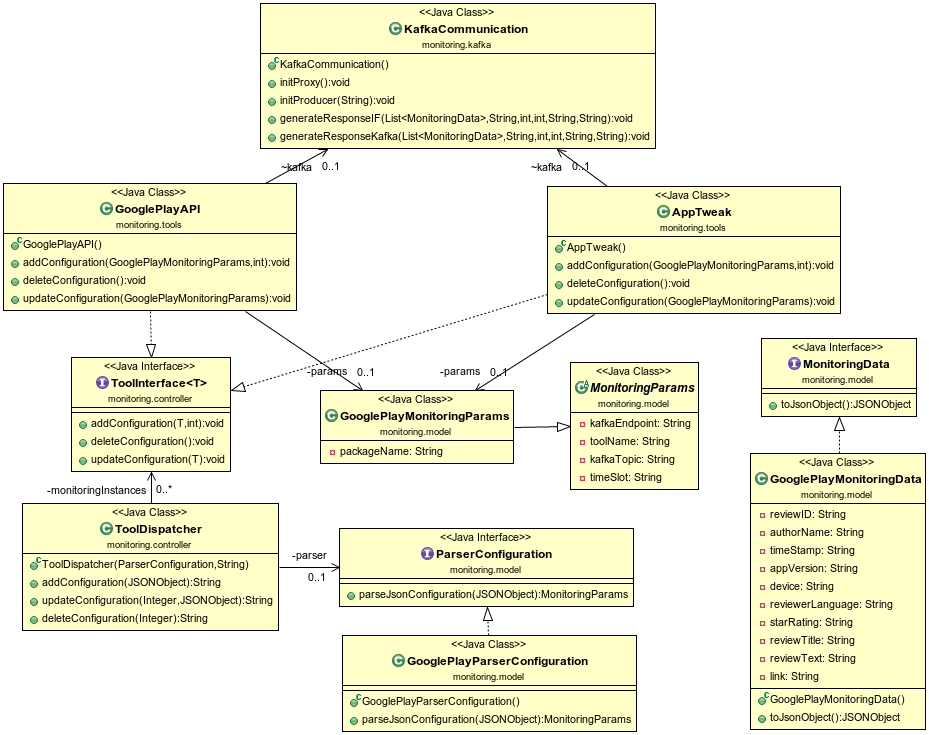
\includegraphics[width=14cm]{Figures/Figure11}
\decoRule
\caption[Arquitectura software del monitor de Google Play]{Arquitectura software del monitor de Google Play}
\label{fig:Figura11}
\end{figure}

La implementació del monitor basada en l'arquitectura genèrica definida presenta diverses similituds en comparació amb el monitor de Twitter, amb la principal diferència que, per aquest cas, tenim 2 \textit{tools} implementades a utilitzar.

\begin{itemize}
\item \textbf{GooglePlayMonitoringParams.} Subclasse de la classe abstracta \textit{MonitoringParams} que hereta els atributs comuns a tots els monitors, i afegeix com a atribut particular del monitor un string \textit{packageName}.
\item \textbf{GooglePlayParserConfiguration.} Implementació de la interfície que defineix la transformació del format d'entrada del monitor (JSONObject) a la instància de \textit{GooglePlayMonitoringParams}.
\item \textbf{GooglePlayMonitoringData.} Implementació de la interfície que defineix la transformació de les dades recollides al format JSON de sortida. En aquest cas hem d'afegir la consideració prèviament introduïda sobre la variabilitat de les dades entre les dues \textit{tools}. Davant aquest punt, podem explotar els avantatges de l'arquitectura presentada, que ens dona dues opcions:
\begin{enumerate}
\item Podem implementar una única classe que estendrà la interfície \textit{MonitoringData} i contindrà tots els paràmetres (comuns i no comuns) de les dades generades durant el procés de monitoratge. En aquest cas, la pròpia \textit{tool} crearà instàncies d'objectes monitorats amb les dades de les quals disposi, i aquelles que no pugui definir (i per tant, que prenguin valors buits o nuls) simplement no apareixeran en la transformació a objecte JSON que enviarem al Kafka \textit{endpoint}. D'aquesta manera, amb una única classe satisfem les necessitats del monitor.
\item Alternativament podem modelar un conjunt de classes que implementin la interfície, de manera que cada \textit{tool} utilitzi una d'aquestes implementacions. D'aquesta manera, disposaríem d'una implementació de \textit{MonitoringData} per cada \textit{tool} d'acord amb la informació que proporciona cadascuna d'aquestes.
\end{enumerate}
\begin{figure}[!h]
\centering
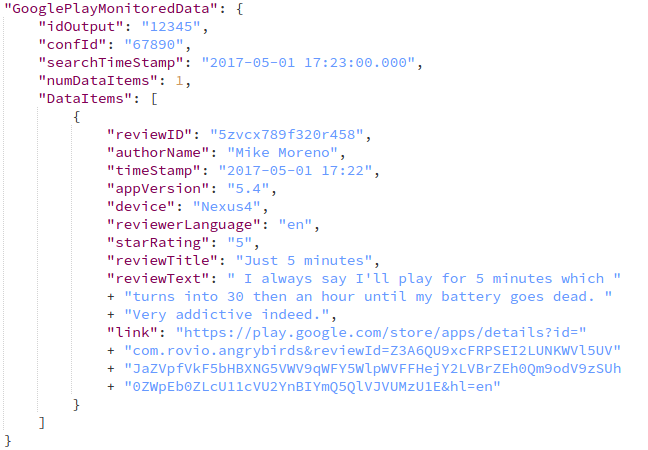
\includegraphics[width=14cm]{Figures/Figure13}
\decoRule
\caption[Exemple dades de sortida generades pel monitor de Google Play]{Exemple dades de sortida generades pel monitor de Google Play}
\label{fig:Figura13}
\end{figure}
Gràcies al disseny, cada desenvolupador podrà utilitzar l'opció que m'es s'adeqüi a les seves necessitats. La 1a opció pot resultar adequada quan p.e. el subconjunt de dades que volem obtenir sigui independent de la \textit{tool}, i per contra la 2a opció ens farà servei per desacoblar totalment les dades entre diferents tools. Pel nostre cas d'ús, considerarem la 1a opció, ja que dins la integració de SUPERSEDE, l'anàlisi d'aquestes dades serà independent de la \textit{tool} utilitzada.
\item \textbf{GooglePlayAPI}. Implementació de \textit{ToolInterface} que utilitza l'API de Google Play Developer. Aquesta \textit{tool} implementa una comunicació mitjançant autenticació OAuth 2.0 mitjançant els \textit{tokens} obtinguts al registrar un usuari de Google Play com a \textit{developer}. Per aquest projecte s'ha utilitzat un compte personal de Google Play compartit amb altres estudiants del Grau en Enginyeria Informàtica, per tal de poder probar i validar aquesta \textit{tool} (ja que, tal i com especificat anteriorment, únicament ens permet obtenir dades de les aplicacions de les quals l'usuari n'és l'autor). Degut al gran volum de dades que es poden generar al demanar les \textit{reviews} d'una aplicació, l'API funciona mitjançant un sistema de paginació. És a dir: la crida REST per obtenir les reviews retorna un subconjunt de mida relativament petita i, addicionalment, un \textit{token} que permet referenciar el següent subconjunt (o pàgina) de reviews. Aquest token s'utilitza per realitzar una nova crida, que conté un nou subconjunt de reviews i, addicionalment, un nou \textit{token} per la següent pàgina. D'aquesta manera, les dades venen paginades i subdividides. És responsabilitat de la \textit{tool} implementar la lògica per realitzar les crides de forma iterativa. 
Aquest tractament pot ser un procés relativament lent (en termes computacionals). Però això no suposa un trencament amb la filosofia de "fotografiar" el sistema en un moment determinat: en el moment que es fa la crida REST, l'API captura les \textit{públiques} en aquell moment, i construeix els objectes de dades paginats, de tal manera que encara que es triguin uns segons en computar totes les pàgines de dades, aquestes sempre seran una representació del moment en que s'ha fet la primera crida, corresponent al final d'un cicle de monitoratge de durada definida al \textit{timeSlot.}
\item \textbf{AppTweak}. Implementació de \textit{ToolInterface} que utilitza l'API de AppTweak. A diferència de l'anterior, tant l'autenticació com la lògica per obtenir les dades és molt més senzilla. En el cas de la primera, funciona mitjançant l'ús d'un \textit{token} a la capçalera de la crida REST, únic per usuari a la plataforma. En el cas de la segona, una sola crida REST retorna totes les dades corresponents a les \textit{reviews} d'aquella aplicació.
\end{itemize}

\noindent{\large{\textbf{Exposició com a servei REST}}}\\

De forma anàloga a l'exposició com a servei del monitor de Twitter, cal dissenyar i implementar un servei REST per desplegar les funcionalitats del monitor de Google Play. La figura ~\ref{fig:Figura14} mostra un exemple d'un possible objecte JSON de configuració del monitor.\\

\begin{figure}[!h]
\centering
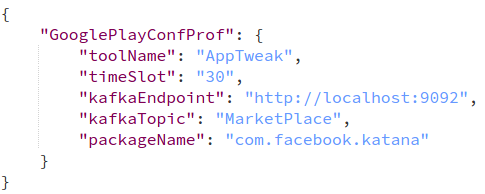
\includegraphics[width=11cm]{Figures/Figure14}
\decoRule
\caption[Exemple JSON de configuració del monitor de GooglePlay]{Exemple JSON de configuració del monitor de GooglePlay}
\label{fig:Figura14}
\end{figure}

Tot i que el paràmetre de \textit{toolName} ja l'havíem vist en l'anterior monitor, ja que és necessari per la instanciació de la \textit{tool} utilitzant el patró reflexió, en aquest cas cobra una especial importància, ja que al disposar d'un conjunt de \textit{tools} podem utilitzar els noms d'aquestes per configurar el monitor; en aquest cas, amb les \textit{tools} de \textbf{GooglePlay} i \textbf{AppTweak}.

\subsubsection{App Store Monitor}

\noindent{\large{\textbf{Exposició com a servei REST}}}\\

\section{Monitor Manager}

Partint de l'arquitectura genèrica dels monitors, i l'exemplificació d'aquesta en casos d'ús reals (i per tant a seva implementació), disposem dels primers components essencials per construïr el nostre sistema. En aquest punt disposem d'un subconjunt de monitors que satisfan les seves especificacions tècniques individuals, relacionades amb l'activitat de monitoratge. Però necessitem anar un pas mes enllà en l'evolució del nostre sistema per satisfer els objectius generals d'adaptabilitat, i procedir a desenvolupar components d'integració.\\

Per aquest objectiu, el primer pas és el desenvolupament del \textbf{Monitor Manager}. Aquest component, tal com el seu nom indica (i com s'ha presentat al \textit{Capítol 5. Visió general del sistema}), s'encarrega de la gestió de tots els monitors desplegats al sistema. Per gestió entenem la satisfacció dels següents requisits funcionals:

\begin{enumerate}
\item \textbf{Inicialització de procés de monitoratge per a un monitor específic.} El component ha de ser capaç de rebre una petició d'inicialització de procés de monitoratge per un dels monitors integrats al sistema, i redireccionar aquesta petició al monitor corresponent, de manera que aquest pugui processar i executar la petició.
\item \textbf{Modificació de procés de monitoratge per a un monitor específic.} Donat un procés de monitoratge existent per a un monitor específic integrat al sistema, el component ha de rebre una petició de reconfiguració d'aquest, processar-la i redireccionar-la al monitor corresponent.
\item \textbf{Aturada de procés de monitoratge per a un monitor específic.} Donat un procés de monitoratge existent per a un monitor específic integrat al sistema, el component ha de rebre una petició per aturar-lo, processar-la i redireccionar-la al monitor corresponent.
\end{enumerate}

Com es pot extreure de les funcionalitats anteriors, l'objectiu principal d'aquest component és \textbf{processar} i \textbf{redireccionar} les peticions relacionades amb accions sobre els monitors desplegats. D'aquesta manera, i enfocat al màxim nivell d'independència entre components, estem afegint un nivell d'abstracció per sobre dels monitors que permetrà la comunicació amb la resta de components del sistema sense necessitat de conèixer els detalls semàntics i tècnics de cada implementació dels monitors.\\

Per tant, com a part de la tasca en el disseny i desenvolupament d'aquest monitor, caldrà definir un punt d'entrada únic pels 3 tipus d'operacions: \textbf{iniciar}, \textbf{modificar} i \textbf{aturar} un procés de monitoratge en un monitor específic. La lògica interna del Monitor Manager, per tant, s'haurà d'encarregar de processar aquestes peticions, identificar a quin monitor pertoca, i redireccionar-la al mateix.

\subsection{Especificacions tècniques}

Les especificacions tècniques en les que ens basarem per dissenyar i implementar el Monitor Manager requereixen satisfer una \textbf{integració} que actuï com a pont \textbf{únic} entre components tercers del sistema i els nostres monitors. Seguint els criteris presentats anteriorment, caldrà considerar els següents punts:

\begin{enumerate}
\item \textbf{INPUT - Petició de configuració de monitor}. Descripció dels paràmetres i el format genèric d'aquests per realitzar la redirecció de la petició.
\item \textbf{\textit{ACTION} - Processat de la petició}. Tractament del format genèric dels paràmetres i interpretació d'acord amb el monitor adreçat.
\item \textbf{\textit{OUTPUT} - Redirecció al monitor}. Enviament de la petició processada cap al monitor.
\end{enumerate}

\subsubsection{INPUT - Petició de configuració de monitor}

La petició de configuració s'ha de rebre en un format genèric que el propi Monitor Manager sigui capaç d'encapsular, identificar el monitor al qual cal enviar-la, i redireccionar-la posteriorment. Per fer-ho, independentment del format, necessitem identificar dos factors claus que el Monitor Manager ha de rebre:

\begin{itemize}
\item El \textbf{monitor específic} al qual s'ha de redireccionar la petició
\item Els \textbf{paràmetres de configuració} per aquell monitor: \textit{toolName} + \textit{kafkaEndpoint} + \textit{kafkaTopic} + \textit{timeSlot} + [paràmetres específics]
\end{itemize} 

Respecte al 2n punt, es tracta d'informació formatada que el monitor específic necessita, i que per tant podem reaprofitar i mantenir estructurada tal i com s'ha documentat prèviament. Respecte al 1r punt, en canvi, es tracta d'informació que el Monitor Manager necessita addicionalment per processar la redirecció.\\

En aquest punt cal decidir si aquesta informació l'afegim de forma implícita a l'objecte JSON de configuració, o bé si busquem una alternativa que ens permeti mantenir l'objecte JSON intacte. En el primer cas, la informació relativa a la configuració queda totalment integrada en un sol objecte JSON que utilitzarem per \textbf{redireccionar} i \textbf{configurar} el monitor. Però això obliga a modificar el format d'aquest JSON, afegint informació addicional que el monitor no necessita. En el segon cas, en canvi, podem mantenir un objecte de configuració que es propaga entre els diferents components: primer com a \textit{input} del Monitor Manager, i després com a \textit{output} redireccionat com a \textit{input} al monitor específic. Alternativament, però, cal buscar una forma de comunicar al Monitor manager a quin monitor trobarà la \textit{tool} sobre la qual hem d'iniciar un procés de monitoratge.\\

\begin{figure}[!h]
\centering
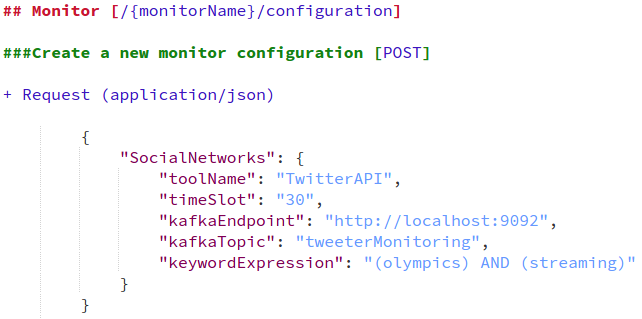
\includegraphics[width=11cm]{Figures/Figure15}
\decoRule
\caption[Exemple JSON de configuració de monitor al Monitor Manager]{Exemple JSON de configuració de monitor al Monitor Manager}
\label{fig:Figura15}
\end{figure}

En aquest sentit aprofitarem la necessitat d'exposició dels components com a serveis RESTful per, mitjançant el propi disseny de la API que implementarà el Monitor Manager, definir aquest paràmetre. En el  disseny d'aquesta API, present a l'apèndix ~\ref{AppendixA}, proposem com a paràmetre dins la URL de les 3 crides a implementar (creació, modificació i eliminació) el propi identificador del monitor. Així, exemplificant la crida per crear una configuració sobre el monitor de Twitter, podem veure a la figura ~\ref{fig:Figura15} la URL que defineix el recurs per realitzar aquesta operació (on \textit{monitorName} és el paràmetre de la URL que identifica el monitor a redireccionar), així com un exemple de JSON que rebrà. Com es pot apreciar, aquest presenta els mateixos camps que el JSON definit als monitors.\\

Amb aquestes dades d'entrada, el Monitor Manager ja és capaç de realitzar la redirecció al monitor corresponent.

\subsubsection{ACTION - Processat de la petició}

Un cop definida la informació i el seu format d'entrada necessaris per satisfer les especificacions tècniques, cal avaluar com partim d'aquesta informació a la petició de configuració de monitors.\\

Ja que la única tasca a realitzar és la redirecció (ja que les dades no cal que siguin tractades), hem de partir del paràmetre \textit{monitorName} per identificar el monitor al qual redireccionar. El component IF exposa, de manera separada, la implementació de classes o \textit{proxies} diferents per cada monitor implementat. És a dir: per cada monitor que vulguem integrar i registrar al nostre sistema, necessitarem afegir-ho a IF per garantir-ne la integració de la comunicació, mitjançant la implementació d'un \textit{proxy} amb els mètodes de comunicació que ofereix. Per tant, la responsabilitat del Monitor Manager serà utilitzar el paràmetre \textit{monitorName} per discernir entre els \textit{proxies} implementats per IF i seleccionar aquell que es correspongui al monitor al qual la petició ha d'anar adreçada. 

\subsubsection{OUTPUT - Redirecció al monitor}

Finalment, identificat i instanciat el \textit{proxy} el Monitor Manager executarà una crida \textit{addConfiguration}, \textit{updateConfiguration} o \textit{deleteConfiguration} en funció de l'operació enviada. De nou en aquest sentit s'aprofita l'\textit{input} d'aquest component mitjançant la seva exposició com a servei: cada mètode de creació, modificació i eliminació crida al mètode corresponent del \textit{proxy} definit per \textit{monitorName}. A aquest \textit{proxy} s'enviarà la instància de configuració rebuda d'entrada, reaprofitant exactament el mateix format, mantenint així la uniformitat de les dades desitjada.

\subsection{Implementació del Monitor Manager}

En definitiva, d'acord amb les necessitats establertes, la implementació del Monitor Manager es basarà simplement en el disseny i implementació d'un servei REST que implementi els 3 mètodes definits anteriorment, i que la seva lògica interna s'encarregui simplement d'identificar, a partir del nom del monitor rebut com a paràmetre, el \textit{proxy} que implementa la comunicació amb aquell monitor.\\

Podeu consultar el projecte i la seva implementació al següent enllaç:  \url{https://github.com/supersede-project/monitor_feedback/tree/develop_quim-motger/monitormanager}

\section{Orchestrator}

Aquest component forma part de la integració d'aquest projecte dins el projecte SUPERSEDE, i per tant el disseny i desenvolupament d'aquest ha estat únicament realitzat com a part d'aquest TFG de forma parcial. Concretament, aquelles parts referents a l'activitat de monitoratge i reconfiguració de monitors.\\

La seva tasca principal és actuar de pont entre els components encarregats d'aplicar adaptacions (\textit{Enactments}) i aquells encarregats del monitoratge (\textit{Monitoring}), que recordem forma part del cicle MAPE-k descrit anteriorment. Aquest és necessari en el moment que diversos sistemes d'adaptabilitat apliquen modificacions en diversos sistemes encarregats de monitorar dades. Aquest TFG n'és un cas específic. Si, per contra, aquest hagués d'actuar com a sistema independent, l'abstracció garantida pel Monitor Manager, que unifica tots els monitors sota un únic punt d'entrada, ja seria suficient per facilitar la comunicació, el manteniment i l'extensió de components. Per contra, si haguéssim volgut afegir la lògica del Monitor Manager al mateix Orchestrator, i aprofitar la seva necessitat dins SUPERSEDE per estalviar-nos una capa en el sistema, ens veuríem obligats a aplicar modificacions i manteniment a l'Orchestrator, un component genèric d'integració, davant modificacions específiques pel nostre cas d'ús. Per tal d'evitar això, s'ha decidit mantenir aquests dos components per separat, i garantir un desacoblament de components el més alt possible.\\

Addicionalment, a aquest component se li assigna una responsabilitat superior associada a la gestió i control del sistema de monitoratge i les seves especificacions. Amb això es fa referència a la persistència i control de metadades relacionades amb els monitors, que ens permeten tenir de forma integrada coneixement sobre el nostre sistema. Aspectes com, p.e., els \textbf{tipus de monitors} integrats, que engloben un conjunt de monitors treballant sobre una mateixa àrea, o bé les \textbf{tools implementades} per cada tipus de monitor.\\

\subsection{Especificacions tècniques}

En general, per tant, podem concebre l'Orchestrator com un \textbf{component d'integració} i un \textbf{repositori de metadades}. Per tant, independentment de les funcionalitats que caldrà implementar (que a continuació detallarem), caldrà tenir en compte dues característiques bàsiques:

\begin{itemize}
\item Haurà de gestionar la \textbf{persistència} de dades relacionades amb els monitors, i per tant caldrà afrontar el \textbf{disseny} i la \textbf{implementació} d'una base de dades.
\item Paral·lelament, caldrà implementar un controlador exposat com a \textbf{servei REST} que exposi les seves funcionalitats i, addicionalment, permeti la seva integració a IF.
\end{itemize}

Per definir els detalls d'aquestes dues branques, necessitem primer definir amb quines metadades estarem treballant i com estructurarem el seu contingut. Definirem, essencialment, tres entitats principals:

\begin{enumerate}
\item \textbf{Monitor configuration}. Instància ja definida anteriorment, que representa l'execució d'una \textit{tool} amb uns paràmetres de configuració específics.
\item \textbf{Monitor tool}. Engloba les metadades associades a aquella \textit{tool} i té associades totes les configuracions en procés d'execució. D'aquesta manera, les dades referents a les configuracions actives per a una \textit{tool} no es troben exclusivament al desplegament del propi monitor, el que suposaria la necessitat d'accedir al propi monitor. Contràriament, aquestes dades es trobaran integrades a l'Orchestrator, el que facilitarà la seva gestió quan es tracti de casos exclusivament de lectura de dades. Aquest darrer propòsit, en qualsevol cas, no entra part del context d'aquest projecte, sinó que està orientat a la integració del TFG amb SUPERSEDE i l'explotació d'aquestes dades.
\item \textbf{Monitor type}. Engloba un conjunt de \textit{tools} que pertanyen a monitors d'una mateixa categoria, com per exemple \textit{Social Networks} o \textit{Market Places}. Aquest agrupament per tipus, com en el cas anterior, tampoc és rellevant pel nostre context, però ens ofereix integració de dades que resulta d'interès en termes analítics.
\end{enumerate}

% Please add the following required packages to your document preamble:
% \usepackage{multirow}
\begin{table}[htb]
\centering
\label{InstanciacioOrchestrator}
\begin{tabular}{|l|l|l|}
\hline
\textbf{Monitor Type}            & \textbf{Monitor Tool}          & \textbf{Monitor configuration} \\ \hline
\multirow{3}{*}{Social Networks} & \multirow{3}{*}{TwitterAPI}    & TwitterAPI-Conf1               \\ \cline{3-3} 
                                 &                                & TwitterAPI-Conf2               \\ \cline{3-3} 
                                 &                                & TwitterAPI-Conf3               \\ \hline
\multirow{6}{*}{Market Places}   & \multirow{2}{*}{GooglePlayAPI} & GooglePlay-Conf1               \\ \cline{3-3} 
                                 &                                & GooglePlay-Conf2               \\ \cline{2-3} 
                                 & GooglePlay-AppTweak            & GooglePlay-AppTweak-Conf1      \\ \cline{2-3} 
                                 & \multirow{2}{*}{iTunesApple}   & iTunesApple-Conf1              \\ \cline{3-3} 
                                 &                                & iTunesApple-Conf2              \\ \cline{2-3} 
                                 & AppStore-AppTweak              & AppStore-AppTweak-Conf1        \\ \hline
\end{tabular}
\caption{Exemple d'instanciació del sistema de monitoratge}
\end{table}

Per tal d'entendre bé aquest esquema, podem visualitzar un esquema conceptual a la taula 7.1 que presenta un exemple de constitució d'un sistema de monitoratge en actiu com el que hem anat descrivint al llarg d'aquest projecte. Bàsicament tenim dos tipus de monitors, \textbf{Social Networks} i \textbf{Market Places}. Pel primer tenim definida una única \textit{tool}, \textbf{TwitterAPI}; pel segon, tenim definides 4, dues per cada \textit{market place} (\textit{AppStore} i \textit{GooglePlay}). Fixem-nos en el detall que en cap moment estem contemplant l'entitat \textbf{monitor} en aquest esquema. Això es deu al fet que, dins el nostre esquema, l'entitat monitor només és significativa des d'un punt de vista físic, com a punt integrat de desplegament que agrupa un conjunt de \textit{tools}. Podríem considerar que existeixen punts comuns entre \textit{tools} dins un mateix monitor, com p.e. la implementació dels paràmetres d'entrada o de sortida. Però la nostra arquitectura no restringeix aquest aspecte. Dins un mateix monitor, cada \textit{tool} pot implementar aquestes interfícies i classes d'acord amb les seves necessitats. D'aquesta manera, el concepte monitor únicament és significatiu des del punt de vista d'implementació i desplegament físic, no lògic o de metadades. Per tant, no considerarem aquesta entitat dins el nostre esquema conceptual.\\

Finalment, a la taula podem veure un conjunt d'exemple de configuracions. Aquest no vindrà limitat per cap restricció, i tot i que cada monitor s'ha d'encarregar en última instància de gestionar-ho, serà a través del Orchestrator i el Monitor Manager que es gestionaran les altes, baixes i modificacions d'aquests.

\subsubsection{INPUT - Peticions de configuració del sistema de monitoratge}

Mitjançant l'exposició de les funcionalitats com a servei REST, l'Orchestrator haurà de rebre el conjunt de peticions amb dos objectius principals: la \textbf{gestió de metadades} del nostre sistema de monitoratge, i la \textbf{redirecció de les peticions} associades directament a configuracions del sistema. La definició d'aquests mètodes d'entrada no ve a ser més que el disseny d'un controlador basat en les operacions \textbf{CRUD} (\textit{\textbf{C}reate}, \textit{\textbf{R}ead}, \textit{\textbf{U}pdate}, \textit{\textbf{D}elete}) per les entitats \textit{Monitor Type}, \textit{Monitor Tool} i \textit{Monitor Configuration}. A la taula 7.2 podem visualitzar un resum conceptual dels mètodes que necessitarem definir, i quins paràmetres caldrà definir per cadascun d'ells.\\

\begin{table}[htb]
\centering
\label{PeticionsOrchestrator}
\begin{tabular}{|p{4cm}|p{6cm}|p{3cm}|}
\hline
\textbf{Operació}                            & \textbf{Definició}                                                        & \textbf{Paràmetres}                                                                                                           \\ \hline
\multicolumn{3}{|c|}{\textbf{Monitor Type}}                                                                                                                                                                                                                        \\ \hline
Llistat de Monitor Types                     & Retorna el llistat de tots els Monitor Types instanciats al sistema       & /                                                                                                                                       \\ \hline
Obté un Monitor Type                         & Retorna les dades d'un Monitor Type específic                             & - nomTipus                                                                                                                              \\ \hline
Alta de Monitor Type                         & Crea una nova instància de Monitor Type                                   & - nomTipus                                                                                                                              \\ \hline
Baixa de Monitor Type                        & Elimina una instància de Monitor Type existent                            & - nomTipus                                                                                                                              \\ \hline
\multicolumn{3}{|c|}{\textbf{Monitor Tool}}                                                                                                                                                                                                                        \\ \hline
Llistat de Tools per Monitor Type            & Retorna el llistat de totes les Tools implementades per a un Monitor Type & - nomTipus                                                                                                                              \\ \hline
Obté una Tool per un Monitor Type            & Retorna les dades d'una Tool per un Monitor Type                          & \begin{tabular}[c]{@{}l@{}}- nomTipus\\ - nomTool\end{tabular}                                                                          \\ \hline
Alta de Tool per un Monitor Type             & Crea una nova Tool per un Monitor Type                                    & \begin{tabular}[c]{@{}l@{}}- nomTipus\\ - nomTool\\ - nomMonitor\end{tabular}                                                           \\ \hline
Baixa de Tool per un Monitor Type            & Elimina una Tool existent per un Monitor Type                             & \begin{tabular}[c]{@{}l@{}}- nomTipus\\ - nomTool\end{tabular}                                                                          \\ \hline
\multicolumn{3}{|c|}{\textbf{Monitor Configuration}}                                                                                                                                                                                                               \\ \hline
Llistat de Configurations per una Tool       & Retorna el llistat de totes les Configurations actives per una Tool       & \begin{tabular}[c]{@{}l@{}}- nomTipus\\ - nomTool\end{tabular}                                                                          \\ \hline
Obté una Configuration per una Tool          & Retorna les dades d'una Configuration per una Monitor Tool                & \begin{tabular}[c]{@{}l@{}}- nomTipus\\ - nomTool\\ - idConf\end{tabular}                                                               \\ \hline
Alta de Configuration per una Tool           & Crea una nova Configuration per una Monitor Tool                          & \begin{tabular}[c]{@{}l@{}}- nomTipus\\ - nomTool\\ - timeSlot\\ - kafkaEndpoint\\ - kafkaTopic\\ - {[}custom{]}\end{tabular} \\ \hline
Modificació d'una Configuration per una Tool & Modifica els paràmetres d'una Configuration existent per una Monitor Tool & \begin{tabular}[c]{@{}l@{}}- nomTipus\\ - nomTool\\ - idConf\\ - timeSlot\\ - kafkaEndpoint\\ - kafkaTopic\\ - {[}custom{]}\end{tabular} \\ \hline                                                                                                                    
Baixa d'una Configuration per una Tool       & Elimina una Configuration existent per una Monitor Tool                   & \begin{tabular}[c]{@{}l@{}}- nomTipus\\ - nomTool\\ - idConf\\ - timeSlot\\ - kafkaEndpoint\\ - kafkaTopic\\ - {[}custom{]}\end{tabular} \\ \hline
\end{tabular}
\caption{Llistat de peticions d'entrada del Orchestrator}
\end{table}

Respecte aquests mètodes, cal considerar els identificadors de cadascuna d'aquestes entitats:

\begin{itemize}
\item \textbf{Monitor Type}. S'identifica per un \textbf{nom} únic
\item \textbf{Monitor Tool}. S'identifica per un \textit{Monitor Type} (un nom de \textit{Monitor Type}) + un \textbf{nom} únic de tool
\item \textbf{Monitor Configuration}. S'identifica per un \textit{Monitor Type} (un nom de \textit{Monitor Type}) + una \textit{Monitor tool} (un nom de \textit{Monitor Tool}) + un \textbf{id} únic de la configuració
\end{itemize}

En general, tota la informació d'entrada que necessita per executar cadascuna de les operacions es basa en identificar el recurs sobre el qual aplicar l'acció. Aquesta identificació a nivell de configuració, que és la darrera entitat que a nosaltres ens interessa considerar, es basa en un triplet de la forma:\\

\centerline{\textbf{monitorType + monitorTool + idConf}}\bigskip

Només en un cas necessitem afegir més informació, que serà pels dos casos a treballar en aquest projecte: la \textbf{creació d'una configuració} i la seva \textbf{reconfiguració} (o actualització). En aquest cas, i tal i com s'ha definit en l'especificació i disseny dels monitors, caldrà afegir d'una banda aquells paràmetres obligatoris per a tot monitor, i addicionalment aquells propis de cada \textit{tool}.\\

\subsubsection{ACTION - Actualització de metadades}

El comportament intern de l'Orchestrator serà relativament senzill, ja que únicament necessita contemplar l'actualització de metadades i el processament de les peticions realitzades per redirigir-les, si s'escau, al monitor corresponent.\\

Considerant primer \textbf{l'actualització de metadades}, l'Orchestrator actualitzarà d'acord a l'operació executada modificacions a la base de dades d'acord amb \textbf{creació}, \textbf{actualització} i eliminació de les entitats prèviament definides. En cas que es tracti d'operacions de lectura, només caldrà accedir a la base de dades i llegir les dades associades a la petició realitzada. Aquest aspecte de l'acció interna el considerarem trivial, ja que es tracta únicament de modificacions associades a una BDD relacional (veure més endavant a \textit{Implementació del Orchestrator}), i no resulta d'especial interès per la finalitat del nostre projecte.\\

\subsubsection{OUTPUT - Redirecció de peticions}

Per altra banda cal definir la \textbf{redirecció de peticions} a monitors. Fixem-nos que, al disposar de totes les dades integrades, aquesta únicament caldrà contemplar-la pels casos en els que no només cal realitzar modificacions sobre les pròpies metadades (o bé simplement realitzar lectures), sinó també realitzar canvis relacionats amb l'execució real dels monitors. Això per tant inclourà: \textbf{alta} de configuració, \textbf{reconfiguració} d'una configuració, i \textbf{eliminació} d'una configuració. En aquests 3 casos, l'Orchestrator haurà de realitzar la redirecció amb el Monitor Manager, utilitzant la integració amb IF.\\

El mateix problema de criteri de redirecció sorgeix que en el cas del Monitor Manager. Necessitem saber quina \textit{tool} va associada a quin monitor, per tal d'indicar al Monitor Manager a quin monitor es troba implementada aquella \textit{tool}. El Monitor Manager requeria aquest paràmetre en la petició, ja que ell no té constància d'aquestes dades. Però a l'Orchestrator sí que disposem d'aquesta metadada, associada a una \textit{tool}, i definida en el moment de creació, tal i com observem també a la taula 7.2. Per tant, a l'hora d'instanciar el \textit{proxy} de IF per comunicar-se amb el Monitor Manager, cridarem al mètode corresponent al Monitor identificat per aquest atribut. D'aquesta manera la redirecció queda satisfeta.\\

\subsection{Implementació de l'Orchestrator}

Sense entrar en molt detall en els aspectes d'implementació de les especificacions prèviament descrites, podem trobar els detalls d'aquesta a: 

\begin{itemize}
\item Disseny de l'esquema de la \textbf{base de dades}, definit a l'apèndix ~\ref{AppendixA}
\item Disseny de l\textbf{API RESTful}, definit a l'apèndix ~\ref{AppendixA}
\end{itemize}

Degut a que el comportament i els detalls específics no són d'especial interés pel domini d'aquest projecte, no s'entrarà amb més detall en la informació referent a la implementació tècnica, que s'ha realitzat seguint les instruccions i els requisits tècnics específics del component Orchestrator genèric implementat per \textit{partners} del projecte SUPERSEDE.
% Chapter Template

\chapter{Sistema d'adaptabilitat} % Main chapter title

\label{DissenySistema} % Change X to a consecutive number; for referencing this chapter elsewhere, use \ref{ChapterX}

Els models UML prèviament descrits ens permeten dissenyar i modelar de forma estandarditzada el sistema de monitoratge. Proporciona, semànticament, tots els recursos necessaris per traduir propostes de configuracions de sistemes en accions reals sobre els monitors implementats.\\

El següent pas és el disseny i implementació d'un sistema que, a partir dels models anteriors, i de tot el domini que defineixen, sigui capaç de gestionar la persistència dels models, obtenir-ne els necessaris per aplicar reconfiguracions, actualitzar els models d'acord a aquestes modificacions, i traduir la informació implícita als models en accions de reconfiguració reals a enviar al sistema de monitoratge.\\

Procedirem a presentar els diferents components que componen aquest sistema.

\section{Model Repository}

El primer component que cal introduir per començar a entendre el \textit{workflow} del sistema d'adaptabilitat és el \textbf{Model Repository}. Aquest component actua en termes genèrics com a un repositori que gestiona la persistència del conjunt de models UML que intervenen en el modelatge del sistema i la seva reconfiguració. Això, per tant, implica tot el conjunt de models descrits anteriorment: \textit{Base Model}, \textit{Feature Model}, \textit{Feature Configuration}, \textit{Pattern Model}, \textit{Profile Model} i \textit{Adaptability Model}.\\

Principalment, les funcionalitats que ha de satisfer són les següents:

\begin{enumerate}
\item Gestionar la persistència dels models en disc
\item Mapejar i encapsular l'estructura de directoris definida per estructurar els models segons el seu tipus
\item Encapsular els mètodes CRUD bàsics per la gestió dels models, aïllant la lògica interna de la resta de components
\item Encapsular mètodes extensius que permetin obtenir models sota unes certes característiques
\end{enumerate}

D'aquesta manera, podem concebre aquest component com una abstracció entre la naturalesa interna dels models i la lògica associada a la càrrega/descàrrega de fitxers amb el nostre sistema, assignant la responsabilitat d'aquests primers punts al Model Repository.\\

Una primera aproximació que ens podríem plantejar seria implementar un component unitari que definís un controlador (que després s'exposaria com a servei per integrar a IF) amb tots els mètodes necessaris per la gestió dels models. Si al nostre sistema únicament resultés d'interès les operacions bàsiques de models, aquesta seria una bona alternativa, ja que estaríem simplificant l'arquitectura del sistema, i hi hauria poc marge per la millora. Però si anem un pas més enllà, i plantegem les necessitats de reconfiguració i adaptabilitat del nostre sistema, veiem que un controlador basat en operacions CRUD únicament ens permetria definir reconfiguracions on tots els models que intervenen en l'adaptació són triats estàticament, no dinàmicament. És a dir: el potencial que oferiria el Model Repository seria referenciar els models implicats en una adaptació mitjançant els seus identificadors, que haurien de ser introduïts manualment.\\

Això per tant implica que no podríem aplicar escenaris d'adaptació com per exemple:\\

\centerline{Actualitzar el sistema de monitoratge amb la darrera Feature Configuration computada}\bigskip

Si tornem al cicle \textit{MAPE-k}, suposant un sistema de \textit{\textbf{P}lanificació} que produeix noves propostes de configuració (FC), aquest enviaria periòdicament aquests models al nostre sistema d'adaptabilitat. Si el nostre sistema és capaç de consultar les dates en què aquestes propostes es van afegint, és capaç de computar quina és la darrera afegida. I en definitiva, és capaç de computar, de forma automàtica i sense necessitat de donar-li cap mena d'informació, quins canvis aplicar al sistema de monitoratge.\\

Aquest escenari és clau pel nostre projecte. L'automatització del nostre sistema ve donada precisament gràcies a la persistència dels models UML i a l'actualització d'aquests, responsabilitat d'un altre sistema, a partir dels quals aquest és capaç de llegir, processar i traduir en modificacions reals sobre les activitats de monitoratge. Aquest escenari, però, és només un exemple de possible escenari d'adaptabilitat, basat en un criteri com la data, que serà el que nosaltres farem servir pel desenvolupament del projecte. Però el potencial està en veure que els criteris poden ser diversos, sempre i quan es treballin amb metadades que podem extreure a partir dels models, com és el cas de la data de generació de les propostes de reconfiguració.\\

Addicionalment a aquest problema, alguns models tenen dependències amb altres models UML. El cas més evident, l'\textit{Adaptability Model}, té dependències amb \textit{Feature Configurations}, que alhora tenen dependències amb \textit{Feature Models}, i també amb \textit{Pattern Models} i \textit{Profile Models}. La resolució i gestió d'aquestes dependències pot arribar a ser extremadament complicada si, al carregar un d'aquests models, necessitem computar i resoldre quines són aquestes dependències cada vegada que volem carregar el Model Repository a memòria per executar una adaptació des del component encarregat d'aquest aspecte, l'Adapter, que satisfent el criteri de distribució del nostre sistema pot no tenir accés al mateix repositori en disc que el Model Repository. \\

Partint d'aquestes necessitats, és evident que necessitem estendre els mètodes de lectura de models a mètodes més complerts, on utilitzem dades auxiliars per fer cerques dins el nostre repositori. És en aquest punt quan aquesta primera aproximació resulta ineficient: si volem accedir a les metadades dels fitxers dels models, tals com la data de creació, l'autor, el sistema que l'ha computat, etc. (més endavant les veurem amb més detall), carregar tots els fitxers dinàmicament per accedir a aquestes dades per fer la cerca resulta molt ineficient. És per això que, alternativament, utilitzarem la següent arquitectura per gestionar la persistència de models:

\begin{itemize}
\item \textbf{Model Repository Manager.} Component que gestiona les metadades dels models, emmagatzemades en una base de dades relacionals, i que estén un controlador amb els mètodes de cerca per obtenir els identificadors dels models associats.
\item \textbf{Model Repository Client.} Component que es comunica amb el Model Repository Manager per obtenir les dades dels models, gestiona la persistència del repositori de models, i encapsula els mètodes i objectes per obtenir i treballar amb els models associats a les reconfiguracions.
\end{itemize}

D'aquesta manera, el primer assumeix les responsabilitats de cerca i gestió de models en base a les seves metadades, i el segon assumeix la responsabilitat principal d'encapsular programàticament l'accés als models, per tal que la resta de components del sistema d'adaptabilitat puguin aïllar-se de la lògica interna d'aquest punt.

\subsection{Model Repository Manager}

Satisfent les necessitats del Model Repository Manager, necessitem contemplar els següents punts:

\begin{enumerate}
\item Disseny i implementació d'una base de dades relacional que emmagatzemi les metadades per cada tipus de model.
\item Disseny i implementació d'un component que accedeixi a la base de dades, i que exposi a través d'un controlador els mètodes de consulta i modificació dels models.
\end{enumerate}

\subsubsection{Disseny de la base de dades}

En primer lloc necessitem definir quines seran les metadades que considerarem per cada model. Generalment, podem considerar que tots els models definits tindran les següents dades:

\begin{itemize}
\item \textbf{Id.} Identificador d'aquell model, únic pel tipus de model (\textit{Base Model}, \textit{Feature Model}...) que representa.
\item \textbf{Name.} Nom del fitxer del model (sense l'extensió).
\item \textbf{AuthorId.} Identificador de l'autor del model.
\item \textbf{CreationDate.} Data de creació del model.
\item \textbf{LastModificationDate.} Data de la darrera modificació del fitxer del model.
\item \textbf{FileExtension.} Extensió del fitxer (.uml, .vql, .yamfc ...)
\item \textbf{SystemId.} Utilitzat dins el context SUPERSEDE per identificar els models que corresponen als diferents escenaris. En el nostre cas, aquest sempre serà \textit{MonitoringReconfiguration}.
\item \textbf{RelativePath.} Ruta relativa del directori \textit{root} on s'emmagatzema el model.
\item \textbf{Dependencies.} Llistat d'identificadors dels models dels quals depèn aquest model.
\end{itemize}

Tot i així, addicionalment existeix la possibilitat d'estendre atributs específics pels diferents models. Considerarem útils pel nostre context els següents:

\begin{itemize}
\item \textbf{Base Model}
\begin{itemize}
\item \textbf{Status.} Indica si el model ha estat computat per un sistema extern (\textit{ComputedByDM}) o bé si és el resultat d'una adaptació dins el sistema d'adaptabilitat (\textit{Enacted}).
\end{itemize}
\item \textbf{Feature Configuration}
\begin{itemize}
\item \textbf{Status.} Ídem que l'atribut al \textit{Base Model}
\end{itemize}
\item \textbf{Adaptability Model}
\begin{itemize}
\item \textbf{Feature Id.} Identificador de la \textit{feature} referenciada per l'Adaptability Model.
\end{itemize}
\end{itemize}

A partir d'aquestes dades podem procedir al disseny de la base de dades del repositori de metadades. Al existir atributs comuns i atributs diferenciats, hem de decidir quin tipus d'herència apliquem a la base de dades. Recordant les tres opcions, aplicades al nostre cas obtindríem el següent:

\begin{itemize}
\item \textbf{\textit{Single table inheritance.}} Definir una única taula a la base de dades \textit{Model} que inclogui tots els atributs possibles, inclosos els específics, i prengui valors nulls per aquells que no tenen aquell atribut.
\item \textbf{\textit{Class table inheritance.}} Definir una taula genèrica \textit{Model} i N taules addicionals per cada tipus que referenciïn la primera, amb els atributs addicionals per cada cas.
\item \textbf{\textit{Concrete table inheritance.}} Definir una taula per cada tipus de model i replicar els atributs comuns.
\end{itemize}

En el nostre cas, optarem per l'opció \textit{concrete table inheritance}. La raó principal d'aquesta opció és que, tot i compartir la major part de les dades, les entitats de models amb tipus diferents mai tindrà sentit contemplar-les conjuntament. És a dir: qualsevol lectura o modificació de models es farà sobre un model (o conjunt de models) d'un tipus específic, mai sobre models de forma genèrica (no tindrà sentit concebir l'entitat \textit{Model} abstracta). Si considerem la segona opció, veiem que seria molt ineficient, ja que caldria fer \textit{joins} internes per obtenir les dades els models, i per la mateixa raó que la ja esmentada sabem que seria un cost innecessari. Per tant, optarem per definir una taula per cada tipus, mantenint així la independència de les metadades entre models. A la figura ~\ref{fig:Figura20} podem veure el disseny proposat de la base de dades, d'acord als 6 tipus de models definits.\\

\begin{figure}
\centering
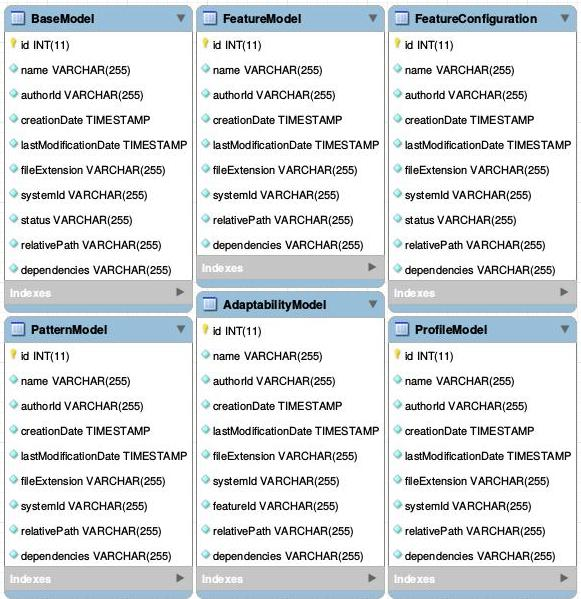
\includegraphics[width=13cm]{Figures/Figure20}
\decoRule
\caption{Disseny de la base de dades del Model Repository Manager}
\label{fig:Figura20}
\end{figure}

\subsection{Model Repository Client}

\section{Adapter}

\section{Model Adapter}

\section{Enactor}

% Chapter Template

\chapter{Validació del sistema} % Main chapter title

Definits els components i detalls que componen el sistema de monitoratge i el sistema d'adaptabilitat, i un cop justificada des d'un punt de vista teòric la satisfacció dels nostres objectius, és el moment de presentar un exemple de cas d'ús i provar l'execució per validar el seu funcionament satisfactori i avaluar els resultats obtinguts.

\section{Presentació de cas d'ús}

Recordem la premissa genèrica del cas d'ús que volem que el nostre sistema satisfaci:

\begin{center}
\textit{Donada un \textbf{procés de monitoratge actiu} en un dels monitors del nostre sistema, i una proposta de \textbf{nova configuració} modelada, volem executar de forma automatitzada una \textbf{reconfiguració} d'aquell procés de monitoratge d'acord amb els \textbf{canvis computats respecte l'actual}.}
\end{center}

Per validar aquesta execució necessitem definir: un \textit{Base Model} que modeli l'estat actual del sistema (figura ~\ref{fig:Figura37}, una \textit{Feature Configuration} que modeli la darrera aplicada al sistema (figura ~\ref{fig:Figura37}, una \textit{Feature Configuration} que modeli la nova proposta de configuració del sistema (figura ~\ref{fig:Figura38}) i un \textit{Adaptability Model} que defineixi l'adaptació de models i la reconfiguració  de monitors (figura ~\ref{fig:Figura39}).\\

\begin{figure}
\centering
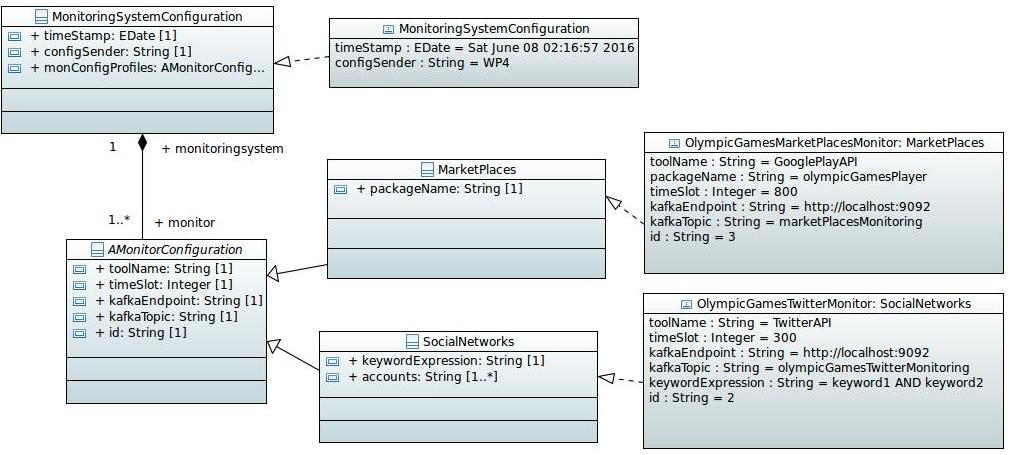
\includegraphics[width=14cm]{Figures/Figure16}
\decoRule
\caption{\textit{Base Model} utilitzat per validar la reconfiguració del sistema}
\label{fig:Figura36}
\end{figure} 

Com podem veure, el \textit{Base Model} defineix una configuració del sistema de monitoratge (ja vista anteriorment com a exemple en el \textit{Capítol 8. Modelatge UML de les configuracions de monitors}) amb dues instàncies de processos de monitoratge corrent: una sobre el monitor de Twitter, i l'altra sobre el monitor de Google Play, ambdues configurades amb els seus propis paràmetres de configuració. Pel nostre cas d'estudi, suposarem que aquest és el darrer \textit{Base Model} que defineix l'estat del sistema.\\

Si ens fixem en les dues \textit{Feature Configuration}, veiem que aquestes són pràcticament les mateixes, a excepció de l'atribut \textit{timeSlot} per les instàncies del monitor de Twitter que, en la nova proposta de configuració, pren un valor més elevat (de 30 segons passa a valer 50). S'ha triat aquest cas d'ús (la modificació del \textit{timeSlot}) per la validació del sistema per dos motius: primerament, per tractar-se d'un cas bàsic que permet observar amb detall la reconfiguració basant-nos en un únic punt de variabilitat, i segon perquè la modificació d'aquest \textit{timeSlot} serà fàcilment visualitzable en el procés d'execució dels monitors.\\ 

Finalment, l'\textit{Adaptability Model} descriu la \textit{feature} timeSlot com a \textit{feature} sobre la qual defineix una adaptació, així com els \textit{patterns} i rols a aplicar sobre els models, i finalment l'acció d'actualització del \textit{timeSlot} d'acord amb el valor definit.\\

\begin{figure}
\centering
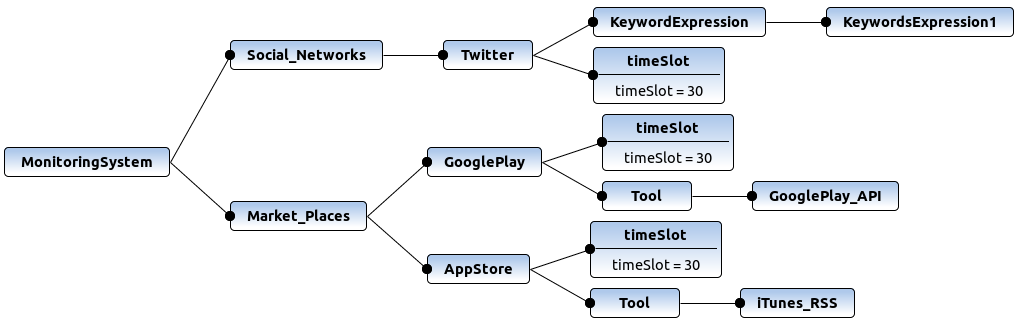
\includegraphics[width=14cm]{Figures/Figure36}
\decoRule
\caption{\textit{Feature Configuration} que descriu la darrera configuració del sistema aplicada}
\label{fig:Figura37}
\end{figure} 

\begin{figure}
\centering
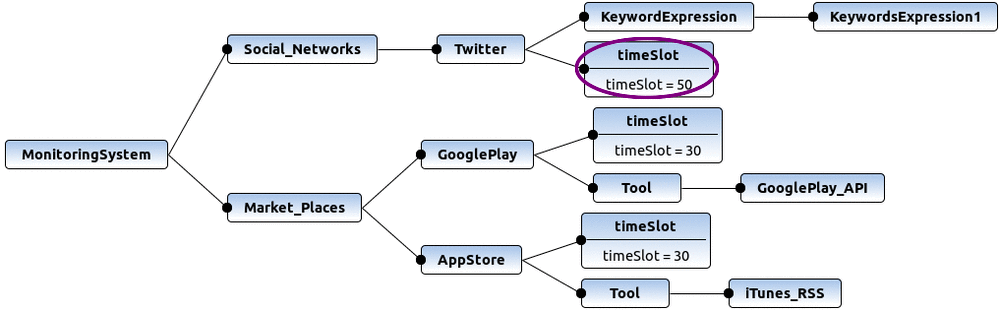
\includegraphics[width=14cm]{Figures/Figure37}
\decoRule
\caption{\textit{Feature Configuration} que descriu la configuració a aplicar per la reconfiguració}
\label{fig:Figura38}
\end{figure} 

\begin{figure}
\centering
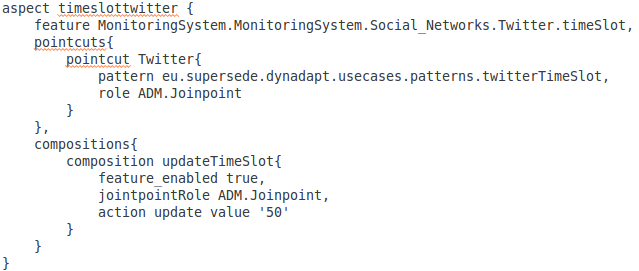
\includegraphics[width=14cm]{Figures/Figure38}
\decoRule
\caption{\textit{Adaptability Model} que descriu la reconfiguració a executar}
\label{fig:Figura39}
\end{figure} 

\section{Execució de la reconfiguració}

El disparador de l'execució serà la sol·licitud a través del \textit{dashboard} de la reconfiguració associada a la \textit{Feature Configuration} 

\begin{figure}
\centering
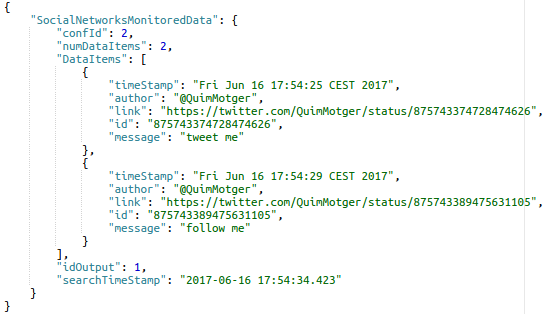
\includegraphics[width=11cm]{Figures/tfg1}
\decoRule
\caption{Primer enviament de dades del monitor de Twitter a Kafka}
\label{fig:tfg1}
\end{figure} 

\begin{figure}
\centering
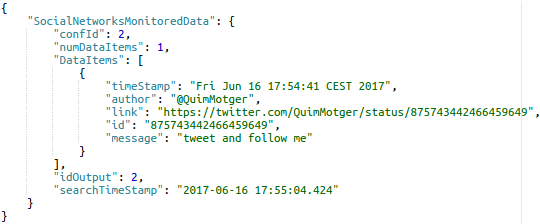
\includegraphics[width=11cm]{Figures/tfg2}
\decoRule
\caption{Segon enviament de dades del monitor de Twitter a Kafka (abans de la reconfiguració)}
\label{fig:tfg2}
\end{figure} 

\begin{figure}
\centering
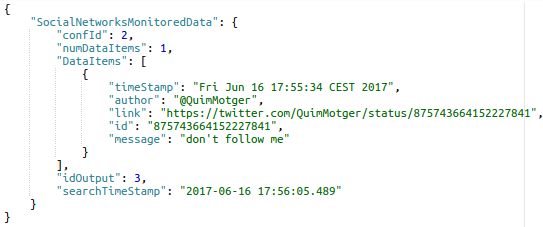
\includegraphics[width=11cm]{Figures/tfg3}
\decoRule
\caption{Tercer enviament de dades del monitor de Twitter a Kafka (després de la reconfiguració)}
\label{fig:tfg3}
\end{figure} 

\begin{figure}
\centering
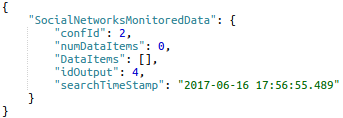
\includegraphics[width=8cm]{Figures/tfg4}
\decoRule
\caption{Quart enviament de dades del monitor de Twitter a Kafka (configuració estable)}
\label{fig:tfg4}
\end{figure} 
% Chapter Template

\chapter{Disseny del dashboard} % Main chapter title

\label{DissenyDashboard} % Change X to a consecutive number; for referencing this chapter elsewhere, use \ref{ChapterX}

%----------------------------------------------------------------------------------------
%	SECTION 1
%----------------------------------------------------------------------------------------

\section{Main Section 1}

Lorem ipsum dolor sit amet, consectetur adipiscing elit. Aliquam ultricies lacinia euismod. Nam tempus risus in dolor rhoncus in interdum enim tincidunt. Donec vel nunc neque. In condimentum ullamcorper quam non consequat. Fusce sagittis tempor feugiat. Fusce magna erat, molestie eu convallis ut, tempus sed arcu. Quisque molestie, ante a tincidunt ullamcorper, sapien enim dignissim lacus, in semper nibh erat lobortis purus. Integer dapibus ligula ac risus convallis pellentesque.

%-----------------------------------
%	SUBSECTION 1
%-----------------------------------
\subsection{Subsection 1}

Nunc posuere quam at lectus tristique eu ultrices augue venenatis. Vestibulum ante ipsum primis in faucibus orci luctus et ultrices posuere cubilia Curae; Aliquam erat volutpat. Vivamus sodales tortor eget quam adipiscing in vulputate ante ullamcorper. Sed eros ante, lacinia et sollicitudin et, aliquam sit amet augue. In hac habitasse platea dictumst.

%-----------------------------------
%	SUBSECTION 2
%-----------------------------------

\subsection{Subsection 2}
Morbi rutrum odio eget arcu adipiscing sodales. Aenean et purus a est pulvinar pellentesque. Cras in elit neque, quis varius elit. Phasellus fringilla, nibh eu tempus venenatis, dolor elit posuere quam, quis adipiscing urna leo nec orci. Sed nec nulla auctor odio aliquet consequat. Ut nec nulla in ante ullamcorper aliquam at sed dolor. Phasellus fermentum magna in augue gravida cursus. Cras sed pretium lorem. Pellentesque eget ornare odio. Proin accumsan, massa viverra cursus pharetra, ipsum nisi lobortis velit, a malesuada dolor lorem eu neque.

%----------------------------------------------------------------------------------------
%	SECTION 2
%----------------------------------------------------------------------------------------

\section{Main Section 2}

Sed ullamcorper quam eu nisl interdum at interdum enim egestas. Aliquam placerat justo sed lectus lobortis ut porta nisl porttitor. Vestibulum mi dolor, lacinia molestie gravida at, tempus vitae ligula. Donec eget quam sapien, in viverra eros. Donec pellentesque justo a massa fringilla non vestibulum metus vestibulum. Vestibulum in orci quis felis tempor lacinia. Vivamus ornare ultrices facilisis. Ut hendrerit volutpat vulputate. Morbi condimentum venenatis augue, id porta ipsum vulputate in. Curabitur luctus tempus justo. Vestibulum risus lectus, adipiscing nec condimentum quis, condimentum nec nisl. Aliquam dictum sagittis velit sed iaculis. Morbi tristique augue sit amet nulla pulvinar id facilisis ligula mollis. Nam elit libero, tincidunt ut aliquam at, molestie in quam. Aenean rhoncus vehicula hendrerit.
% Chapter Template

\chapter{Validació del sistema} % Main chapter title

\label{ValidacioSistema} % Change X to a consecutive number; for referencing this chapter elsewhere, use \ref{ChapterX}

%----------------------------------------------------------------------------------------
%	SECTION 1
%----------------------------------------------------------------------------------------

\section{Main Section 1}

Lorem ipsum dolor sit amet, consectetur adipiscing elit. Aliquam ultricies lacinia euismod. Nam tempus risus in dolor rhoncus in interdum enim tincidunt. Donec vel nunc neque. In condimentum ullamcorper quam non consequat. Fusce sagittis tempor feugiat. Fusce magna erat, molestie eu convallis ut, tempus sed arcu. Quisque molestie, ante a tincidunt ullamcorper, sapien enim dignissim lacus, in semper nibh erat lobortis purus. Integer dapibus ligula ac risus convallis pellentesque.

%-----------------------------------
%	SUBSECTION 1
%-----------------------------------
\subsection{Subsection 1}

Nunc posuere quam at lectus tristique eu ultrices augue venenatis. Vestibulum ante ipsum primis in faucibus orci luctus et ultrices posuere cubilia Curae; Aliquam erat volutpat. Vivamus sodales tortor eget quam adipiscing in vulputate ante ullamcorper. Sed eros ante, lacinia et sollicitudin et, aliquam sit amet augue. In hac habitasse platea dictumst.

%-----------------------------------
%	SUBSECTION 2
%-----------------------------------

\subsection{Subsection 2}
Morbi rutrum odio eget arcu adipiscing sodales. Aenean et purus a est pulvinar pellentesque. Cras in elit neque, quis varius elit. Phasellus fringilla, nibh eu tempus venenatis, dolor elit posuere quam, quis adipiscing urna leo nec orci. Sed nec nulla auctor odio aliquet consequat. Ut nec nulla in ante ullamcorper aliquam at sed dolor. Phasellus fermentum magna in augue gravida cursus. Cras sed pretium lorem. Pellentesque eget ornare odio. Proin accumsan, massa viverra cursus pharetra, ipsum nisi lobortis velit, a malesuada dolor lorem eu neque.

%----------------------------------------------------------------------------------------
%	SECTION 2
%----------------------------------------------------------------------------------------

\section{Main Section 2}

Sed ullamcorper quam eu nisl interdum at interdum enim egestas. Aliquam placerat justo sed lectus lobortis ut porta nisl porttitor. Vestibulum mi dolor, lacinia molestie gravida at, tempus vitae ligula. Donec eget quam sapien, in viverra eros. Donec pellentesque justo a massa fringilla non vestibulum metus vestibulum. Vestibulum in orci quis felis tempor lacinia. Vivamus ornare ultrices facilisis. Ut hendrerit volutpat vulputate. Morbi condimentum venenatis augue, id porta ipsum vulputate in. Curabitur luctus tempus justo. Vestibulum risus lectus, adipiscing nec condimentum quis, condimentum nec nisl. Aliquam dictum sagittis velit sed iaculis. Morbi tristique augue sit amet nulla pulvinar id facilisis ligula mollis. Nam elit libero, tincidunt ut aliquam at, molestie in quam. Aenean rhoncus vehicula hendrerit.
% Chapter Template

\chapter{Treball futur i possibles expansions} % Main chapter title

\label{TreballFutur} % Change X to a consecutive number; for referencing this chapter elsewhere, use \ref{ChapterX}


% Chapter Template

\chapter{Conclusions} % Main chapter title

\label{Conclusions} % Change X to a consecutive number; for referencing this chapter elsewhere, use \ref{ChapterX}

Com a cloenda pel desenvolupament d'aquest projecte, aquest darrer capítol pretén recollir una avaluació general del producte generat, la feina desenvolupada, el seu potencial i en definitiva, resumir tots els aspectes que engloben el desenvolupament d'un TFG d'aquestes característiques.

\section{Justificació de l'assoliment de competències}

Com a part de la planificació del projecte i el curs de GEP, es van definir una sèrie de competències que es treballarien en aquest projecte en diferents graus. Un cop finalitzat el seu desenvolupament, hem d'assegurar no només la satisfacció dels objectius (plantejada al \textit{Capítol 11. Validació del sistema}), sinó també d'aquestes competències i el seu treball amb el màxim rigor possible.

\begin{enumerate}
\item [CES1.1.] \textbf{Desenvolupar, mantenir i avaluar sistemes i serveis software complexos i/o crítics. [En profunditat]}
\subitem L'objectiu principal del projecte ha estat el desenvolupament de dos sistemes (de monitoratge i d'adaptabilitat) formats per un conjunt de components independents, integrats entre ells per satisfer un objectiu major. El desenvolupament de cadascun d'aquests components, així com el seu disseny, el seu \textit{testing} i la seva validació han suposat un treball en profunditat del treball realitzat en un sistema software complex, amb un ús de tecnologies variat i amb requisits diferenciats.
\item [CES1.2.] \textbf{Donar solució a problemes d'integració en funció de les estratègies, dels estàndards i de les tecnologies disponibles. [En profunditat]}
\subitem La integració i comunicació d'aquests components s'ha dissenyat i desenvolupat al llarg del projecte. La necessitat de disposar d'un sistema distribuït ens ha presentat la necessitat de donar solució a la integració de components, d'una banda a través de la necessitat del component d'integració utilitzat (IF), i d'altra banda el disseny i implementació de la lògica necessària a cada component per ser exposat com a servei i poder ser així integrat a IF.
\item [CES1.3.] \textbf{Identificar, avaluar i gestionar els riscos potencials associats a la construcció de software que es poguessin presentar. [Bastant]}
\subitem Especialment treballada durant la planificació del projecte, i utilitzada durant el seu desenvolupament, la gestió i planificació temporal s'ha adaptat a les petites desviacions que s'han anat patint al llarg del desenvolupament.
\item [CES1.5.] \textbf{Especificar, dissenyar, implementar i avaluar bases de dades.  [Bastant]}
\subitem Components com l'Orchestrator o el Model Repository Manager han necessitat l'especificació, el disseny, la implementació i l'avaluació de bases de dades relacionals. Aquestes tasques s'han realitzat d'acord a les necessitats de cada component.
\item [CES1.7.] \textbf{Controlar la qualitat i dissenyar proves en la producció de software. [En profunditat]}
\subitem Tots els components han estan validats independentment per satisfer la seva funcionalitat satisfactòriament; addicionalment, es dedica el \textit{Capítol 11. Validació del sistema} per controlar i avaluar l'execució completa de tots els components dins el \textit{workflow} d'adaptació del sistema de monitoratge.
\item [CES1.8.] \textbf{Desenvolupar, mantenir i avaluar sistemes de control i de temps real. [En profunditat]}
\subitem Els monitors implementats són components que interactuen en temps reals amb altres sistemes software. Aquests components s'han dissenyat i desenvolupat en el context d'aquest projecte, i ha calgut també la seva validació per permetre la seva integració.
\item [CES1.9.] \textbf{Demostrar comprensió en la gestió i govern dels sistemes software. [En profunditat]}
\subitem Al llarg de tot el projecte s'ha plantejat un fil conductor per descriure els diferents components a implementar i com els requisits del sistema s'han anat satisfent amb el desenvolupament d'aquests. Addicionalment s'han incorporat els raonaments i justificacions pertinents, tant per ajudar al lector a entendre el procés de desenvolupament, com per demostrar l'assimilació dels coneixements de gestió del sistema software generat.
\item [CES2.1.] \textbf{Definir i gestionar els requisits d'un sistema software. [En profunditat]}
\subitem Satisfet en la part de la planificació, des d'un punt de vista genèric per tot el sistema, i addicionalment durant el desenvolupament del projecte, conforme de cada component hem extret els requisits necessaris per procedir al seu desenvolupament.
\item [CES2.2.] \textbf{Dissenyar solucions apropiades en un o més dominis d'aplicació, utilitzant mètodes d'enginyeria del software que integrin aspectes ètics, socials, legals i econòmics. [Bastant]}
\subitem El \textit{Capítol 4. Gestió i desenvolupament} presenta d'una banda un anàlisi detallat i numèric dels requisits econòmics del projecte, segons criteris com les hores necessàries, l'equip físic i humà, etc. Per altra banda, presenta l'anàlisi dels criteris de sostenibilitat des del punt de vista ètic, social i legal que al llarg de tot el projecte s'ha assegurat que es garanteixen
\textbf{\item [CES3.1.] Desenvolupar serveis i aplicacions multimèdia. [En profunditat]}
\subitem L'exposició de tots els components com a serveis RESTful per permetre la seva integració, o bé el desenvolupament del \textit{dashboard} per l'adaptabilitat del sistema, ha suposat no només el treball d'aquests coneixements en aquest projecte, sinó també un aprenentatge en desenvolupament d'APIs i \textit{front-end}.
\end{enumerate}

\section{Avaluació del potencial del producte generat}

Els resultats generats i el potencial de cadascun dels components desenvolupats s'han anat tractant i presentant al llarg del projecte, però és convenient fer un resum sobre el potencial del producte generat de cara a desenvolupament futur i ampliació de les seves funcionalitats.\\

Primerament, la \textbf{proposta d'una arquitectura genèrica} pel desenvolupament de monitors obre la possibilitat d'extensió del sistema de monitoratge amb relativa facilitat, partint de la documentació que aquesta mateixa memòria presenta. De fet, actualment altres col·laboradors del projecte han fet servir aquesta mateixa arquitectura per desenvolupar altres monitors que s'han integrat en el sistema SUPERSEDE per altres casos d'estudi. Això és un exemple de com aquesta proposta satisfà el nostre objectiu d'heterogeneïtat, i permet partint d'una arquitectura genèrica implementar un monitor reutilitzant el màxim dels components, i assumint com a única responsabilitat addicional del desenvolupador la lògica interna del monitor.\\

Respecte al sistema d'adaptabilitat, la validació d'aquest projecte es centra en la reconfiguració de processos de monitoratge actius, però els components desenvolupats i el model d'adaptació obre la porta a una \textbf{autonomia total del sistema} i una reconfiguració molt més completa. El sistema dona suport a modificacions més complexes de models UML, com per exemple afegir instàncies de configuracions (processos de monitoratge). Amb poques modificacions, podríem estendre i definir adaptacions molt més complexes: el sistema de monitoratge suporta completament qualsevol operació respecte els processos de monitoratge, i dins el sistema d'adaptabilitat, només caldria definir els models de configuració que defineixin aquests canvis, i adaptar el component Enactor per suportar la traducció a aquest tipus de peticions. Així, a mesura que es treballi en noves configuracions, podem disposar d'un sistema que no només sigui autoadaptable des del punt de vista de reconfiguració de processos de monitoratge, sino fins i tot en la posada en marxa i aturada.\\

Finalment, cal contemplar que aquest projecte ha estat desenvolupat centrant-se en el cas de reconfiguració de monitors, però sempre respectant la seva integració dins SUPERSEDE. Això ha permès que alguns dels components desenvolupats, com per exemple el Model Repository, l'Adapter o el Model Adapter són completament reutilitzables per altres casos d'estudi totalment independents a la reconfiguració de monitors. En cada cas, caldria plantejar les necessitats de models, i estendre el Model Adapter per suportar l'adaptació dels models definits. A partir d'aquí, des d'un punt de vista genèric, la reconfiguració de sistemes és totalment autònoma i abstracta a la necessitat del sistema.\\

En resum, podem satisfer que per una banda s'ha resolt una problemàtica específica, alhora que el producte generat permet el seu ús i reutilització per seguir treballant i desenvolupar en resoldre problemes dins la mateixa àrea i amb objectius similars.

\section{Avaluació general}

Davant els punts anteriorment exposats, es pot garantir no només la satisfacció dels objectius propis del projecte, sinó també els objectius des d'un punt de vista didàctic com a projecte que representa la cloenda dels estudis del Grau en Enginyeria Informàtica.\\

Aquest projecte ha suposat, a títol personal, una de les primeres experiències en el desenvolupament d'un projecte amb implicacions reals, entenent aquest desenvolupament com el transcurs en la seva totalitat: des del plantejament de les necessitats i requisits fins la seva validació, passant pel disseny software i la implementació dels components especificats. Com a futur professional de l'enginyeria del software, l'oportunitat de participar en aquestes fases d'un projecte i veure la seva evolució aporta un gran valor personal i professional, que serveix de perfecte tancament dels estudis mitjançant l'assoliment i validació final dels coneixements adquirits durant el transcurs del grau.\\

Addicionalment aquest projecte ha suposat no només una consolidació dels coneixements adquirits, sinó també un aprenentatge de tecnologies o conceptes que altrament és probable que no hagués tractat. Degut a la gran variabilitat de requisits tècnics dels diferents components del projecte, ha estat necessari afrontar reptes variats que en alguns casos han suposat dedicar hores d'aprenentatge (com, p.e., el disseny d'un \textit{front-end} amb un \textit{framework} específic). Aquest és un punt essencial que, a més, reflexa perfectament la realitat del món laboral dins el sector de l'enginyeria informàtica: la constant necessitat de renovació i aprenentatge en funció de les circumstàncies del moment.\\

En definitiva les sensacions al finalitzar aquest projecte són altament satisfactòries. Consolidant els coneixements interioritzats durant els 4 anys d'aquest grau, produeix una gran motivació veure d'una banda les habilitats i coneixements adquirits, i d'altra banda el potencial coneixement encara per adquirir i desenvolupar, ja sigui en altres entorns acadèmics o en el món laboral. És el moment de tancar el darrer capítol d'aquesta memòria i, amb sort, començar a escriure'n molts més allà on el futur professional em condueixi. \\

%----------------------------------------------------------------------------------------
%	THESIS CONTENT - APPENDICES
%----------------------------------------------------------------------------------------

%\appendix % Cue to tell LaTeX that the following "chapters" are Appendices

% Include the appendices of the thesis as separate files from the Appendices folder
% Uncomment the lines as you write the Appendices

%% Appendix A

\chapter{Frequently Asked Questions} % Main appendix title

\label{AppendixA} % For referencing this appendix elsewhere, use \ref{AppendixA}

\section{How do I change the colors of links?}

The color of links can be changed to your liking using:

{\small\verb!\hypersetup{urlcolor=red}!}, or

{\small\verb!\hypersetup{citecolor=green}!}, or

{\small\verb!\hypersetup{allcolor=blue}!}.

\noindent If you want to completely hide the links, you can use:

{\small\verb!\hypersetup{allcolors=.}!}, or even better: 

{\small\verb!\hypersetup{hidelinks}!}.

\noindent If you want to have obvious links in the PDF but not the printed text, use:

{\small\verb!\hypersetup{colorlinks=false}!}.

%\include{Appendices/AppendixB}
%\include{Appendices/AppendixC}

%----------------------------------------------------------------------------------------
%	BIBLIOGRAPHY
%----------------------------------------------------------------------------------------

\setquotestyle{english}
\printbibliography[heading=bibintoc]

%----------------------------------------------------------------------------------------

\end{document}  
